% erstellt am 2015-07-18 von Jan Dreyling-Eschweiler
\documentclass[pdftex, a4paper, 12pt, oneside]{scrbook}  % oneside skip one blank page before new chapter

% für Umlaute im Quelltext, ngerman und german haben unterschiedliche Trennungsregeln 
\usepackage[ngerman]{babel}
\usepackage[utf8]{inputenc}
\usepackage[T1]{fontenc}

\usepackage{amssymb,amsmath}
\usepackage[font=small,format=plain,labelfont=bf,up]{caption} % fuer kleinere caption

%\usepackage{subfigure}
\usepackage{subcaption}
\usepackage{wrapfig}
\usepackage{sidecap}

\usepackage{natbib}

\usepackage{array}
\usepackage{geometry}
\geometry{includehead,includefoot,inner=4cm,outer=3cm,top=2.5cm,bottom=2.5cm} % test layout

\usepackage{txfonts} % serif font
\setkomafont{sectioning}{\bfseries} % section als in serif

\usepackage{hyperref} % fuer links[hidelinks]
\usepackage{supertabular} % fuer tabellen ueber mehrere seiten
\usepackage{pbox}
\usepackage{sidecap}
\usepackage{multirow} % zum verbinden von tabellenzellen, vertikal
\usepackage{mathrsfs} % fuer \mathscr{L} 

%% pdftex 
%\pdfcompresslevel=1
%\pdfimageresolution=40

%\usepackage{mdwlist} % using “compacted” lists, \begin{itemize*}

\usepackage{enumitem} % also for compact list

\usepackage{setspace}

% drawings
\usepackage{tikz}
\usetikzlibrary{arrows}

%appendix
\usepackage[title,titletoc]{appendix}

%different tocdepth
\usepackage{tocvsec2}

% extra content
\usepackage{titletoc}

% stretch tables
\renewcommand{\arraystretch}{1.5}

% einzug fussnoten
\usepackage[hang]{footmisc}
\setlength{\footnotemargin}{-0.8em}

\usepackage[acronym,toc]{glossaries}
\makeglossaries
\newglossaryentry{abroller}{
name={Abroller},
description={Eine Schußtechnik, bei dem die Stange durch Abrollen der Handfläche gedreht wird. Siehe auch Pin.}
}

\newacronym{dtfb}{DTFB}{Deutscher Tischfußball Bund}


\newacronym{offensive}{Offensive}{Spielaktionen mit Ballbesitz: Passen und Schiessen}
\newacronym{defensive}{Defensive}{Spielaktionen und Stellungsspiel ohne Ballbesitz}


\usepackage{nameref}

% abstand von item 
%\newlength{\wideitemsep}
%\setlength{\wideitemsep}{0.5\itemsep}
%\addtolength{\wideitemsep}{-3pt}
%\let\olditem\item
%\renewcommand{\item}{\setlength{\itemsep}{\wideitemsep}\olditem}

%\setlength{\itemsep}{0pt}

\setitemize{itemsep=-2pt,topsep=2pt}
\setenumerate{itemsep=-2pt,topsep=2pt}

\setlength{\bibsep}{5pt}
% further option
\setlength{\parindent}{15pt} % stell den absatz einzg ein z.b. auch null
%\setlength{\parskip}{4pt} % legt den abstand zwischen paragraphen fest, aber auch aufzählungen oder so...

% globale trennung
%\hyphenation{}

% no vertical stretch
\raggedbottom %instead of default flushbottom


%%%%%%%%%%%%%%%%%%%%%%%%%%%%%%%%%%%%%%%%%%%%%%%%%%%%%%%%%%%%%%%%%%%%%%
%%%%%%%%%%%%%%%%%%%%%%%%%%%%%%%%%%%%%%%%%%%%%%%%%%%%%%%%%%%%%%%%%%%%%%
%%%%%%%%%%%%%%%%%%%%%%%%%%%%%%%%%%%%%%%%%%%%%%%%%%%%%%%%%%%%%%%%%%%%%%
\begin{document}


%%%%%%%%%%%%%%%%%%%%%%%%%%%%%%%%%%%%%%%%%%%%%%%%%%%%%%%%%%%%%%%%%%%%%%
% title page
\title{Tischfußball-Grundlagen}
\author{DTFJ Team}
\newcommand*{\titlebskfactor}{0.68}

\makeatletter
\begin{titlepage}
  \rule{\textwidth}{0pt}
  \vfill
  \begin{center}
    \normalfont \bfseries
    \begin{spacing}{1.2}
      \Huge \@title
    \end{spacing}

    \vspace{1cm}

    {
      \Large Ein Dokument
      \\[\titlebskfactor\baselineskip]
      zum Spielen und Erlernen 
      \\[\titlebskfactor\baselineskip]
      von Tischfußball
      \\[\titlebskfactor\baselineskip]
    }

    \vspace{0.5cm}
    
    \begin{minipage}{0.5\textwidth}
	\centering
	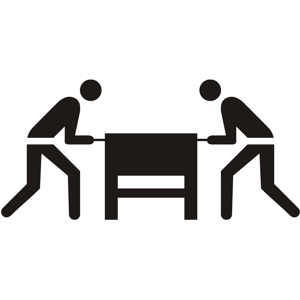
\includegraphics[width=0.8\textwidth]{img/logos/tischfussball.jpg}
    \end{minipage}%
%    \begin{minipage}{0.5\textwidth}
%	\centering
%	
\includegraphics[width=0.7\textwidth]{img/logos/DTFJ_Logo.jpg}
%    \end{minipage}

    \vspace{0.5cm}

    {
%      \large Zusammengestellt vom 
%      \\[\titlebskfactor\baselineskip]
%      \@author
%      \\[\titlebskfactor\baselineskip]
%      \vspace{.5cm}
      November 2015
    }

  \end{center}
  \vfill
  \vfill
\end{titlepage}
\makeatother



%%%%%%%%%%%%%%%%%%%%%%%%%%%%%%%%%%%%%%%%%%%%%%%%%%%%%%%%%%%%%%%%%%%%%%
% Inhalt %%%
\cleardoublepage 
\newpage

% page numbering
\pagenumbering{arabic}
\setcounter{page}{1}

% contents
\setcounter{secnumdepth}{3} % Nummerierungstiefe
\setcounter{tocdepth}{3} % Anzeigetiefe
\renewcommand{\contentsname}{Inhalte}
\tableofcontents


%%%%%%%%%%%%%%%%%%%%%%%%%%%%%%%%%%%%%%%%%%%%%%%%%%%%%%%%%%%%%
% Text 
\cleardoublepage
\thispagestyle{empty}

%%%%%%%%%%%%%%%%%%%%%%%%%%%%%%%%%%%%%%%%%%%%%%%%%%%%%%%%%%%%%
% abstract 
\addcontentsline{toc}{chapter}{Vorwort}
\chapter*{Vorwort}

% Warum?
Tischfußball-Status? Ziele?
% 
Kurze Beschreibung der Inhalte dieses Dokuments.



%%%%%%%%%%%%%%%%%%%%%%%%%%%%%%%%%%%%%%%%%%%%%%%%%%%%%%%%%%%%%
% einleitung 
\chapter{Einleitung}

\section{Spielprinzip}

\begin{itemize}
\item Fußball auf einem Tisch.
\item Tore schiessen
\item Durch Bewegen und Drehen der Stangen können Spielfiguren den Ball beeinflussen und spielen
\end{itemize}

\section{Mehr als nur ein Spiel}

\begin{itemize}
\item Spiel für jedermann und jederfrau, für Alt und Jung. 
\item Soziale Aspekte: Zusammenkommen und Kennenlernen, modernes Vereinsleben.
\item Individuelle Entwicklung: Motorik, Konzentration, Verlieren lernen
\end{itemize}

\section{Tischfußball als Sport}

\begin{itemize}
\item Vereine und Verbände
\item Einzel, Doppel, Team
\item Turniere und Ranglisten
\item Weltmeisterschaften, Deutsche Meisterschaften, Landesmeisterschaften, ...
\end{itemize}



%%%%%%%%%%%%%%%%%%%%%%%%%%%%%%%%%%%%%%%%%%%%%%%%%%%%%%%%%%%%%
% sportgerät und zubehör
\chapter{Spielgerät und Zubehör}
\label{tisch}


%%%%%%%%%%%%%%%%%%%%%%%%%%%%%%%%%%%%%%%%%%%%%%
\section{Der Tisch}
\label{tisch:tisch}

Der Tisch zusammen mit einem Ball ist das Spielgerät beim Tischfußball. 
Das etwa 1,1 m lange und 0,7 m breite Spielfeld ist im Tischkorpus, der auf vier Beinen steht, eingelassen und von Banden umrundet. An den Stirnseiten sind die Tore platziert, die mit einer Torauffangschale oder einem Ballrücklauf ausgestattet sind.  
Die jeweils 11 Spielfiguren sind auf 4 Stangen (für drei Spielbereiche) verteilt:
\begin{itemize}  
    \item die Torwartstange, auch Torwart (\gls{abwehr}) 
    \item die 2er-Stange, auch die Zwei (\gls{abwehr}) 
    \item die 5er-Stange, auch die Fünf (\gls{mittelfeld})
    \item die 3er-Stange (\gls{sturm})
\end{itemize}  
Die Stangen können mittels Griffen vor- und zurückgedreht und rein- und rausgeschoben werden.
Wenn man am Tisch steht, ist die Spielrichtung von links nach rechts, also das linke Tor ist das eigene und das rechte Tor das vom Gegner.
Neben diesem Grundaufbau, der in der Abbildung \ref{fig:tisch:tischbereiche} verdeutlicht wird, gibt es einige kleinere Unterschiede bei den vielen \nameref{tisch:tisch:modelle}n. 

\begin{figure}
    \centering 
    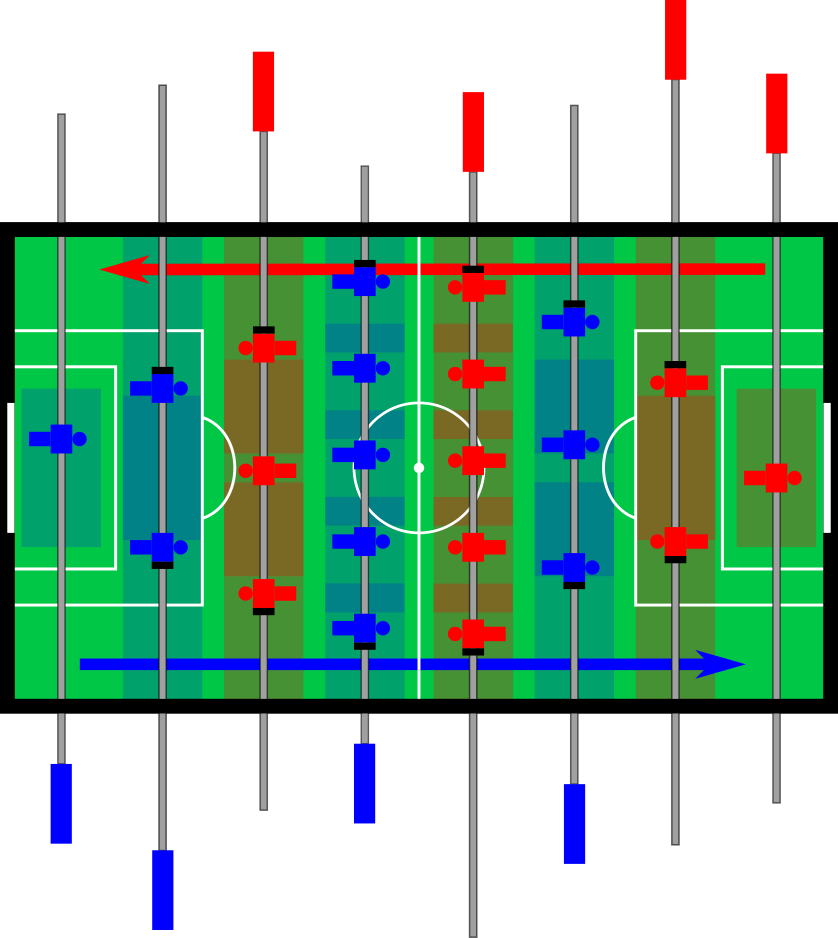
\includegraphics[width=0.9\textwidth]{img/grundlagen_bereiche2.png}
    \caption{Die Grundaufstellung eines Tischfussball-Tischs. Die Pfeile deuten die Vorwärts-Spielrichtung der jeweiligen Seite -- rot oder blau -- an. In den vertikal eingedunkelten Bereichen können die Figuren der jeweiligen Stange einen Ball erreichen. Die dunkleren Bereiche können von den jeweiligen beiden nächsten Figuren erreicht werden.} 
    \label{fig:tisch:tischbereiche} 
\end{figure}

\subsection{Tischmodelle}
\label{tisch:tisch:modelle}

Inzwischen gibt es Tischmodelle vieler Hersteller in allen Qualitäts- und Preis-Kategorien:
\begin{itemize}
    \item günstige, aber auch billige Tische gibt es schon ab 100 Euro 
    \item qualitiative Tische für Hobbyspieler gibt es ab 300-600 Euro
    \item Trainingstische für Turnierspieler gibt es ab 600-1.200 Euro
    \item offizieller Turniertische gibt es ab 1.200 Euro 
\end{itemize}

Letztendlich sollte der Tisch dem Spielniveau angemessen sein, damit der Spielspaß hochgehalten wird. Dennoch gibt es ein paar Grundsätze, die man beispielsweise bei einem Tischkauf beachten sollte:
\begin{itemize}
    \item Der Korpus sollte ein gewisses Gewicht haben, damit er nicht leicht verrutscht. Turniertische beispielsweise wiegen über 100 kg.
    \item Die Beine sollten nicht wackeln und höhenverstellbar sein.
    \item Die Stangen sollten sich nicht leicht verbiegen lassen.
    \item {\normalfont \bfseries Empfehlung:} Bei einer Anschaffung eines Tisches und von Bällen sollte man darauf achten, dass ein griffiges Ball-Handling das anfängliche Erlernen eines kontrollierten Spiels signifikant erleichtert.
\end{itemize}

In Tabelle \ref{tab:tische} werden die Merkmale und Unterschiede der 5 offiziellen Tischmodelle des \gls{itsf} und der zwei weiteren Partnertische des \gls{dtfb} verglichen. 
Die Angaben in der Tabelle beziehen sich auf das jeweilige offizielle Turniermodell, jedoch hat jeder dieser Tischhersteller vergleichbare Modelle für den Anfänger, Jugend- oder Hobbyspieler. 
Zusätzliche Unterschiede sind bei einigen Modellen das verkürztes Spielfeld, was ein hohes Tor erfrdert und den Fahrweg des Torwarts verkürzt.
Beim amerikanischen Modell Tornado hat die Torwartstange ebenfalls drei Figuren, da die Ecken nicht schräg sind und so Bälle in diesem Bereich gespielt werden können.
Weitere Infos gibt es hier:
\begin{itemize}
    \item \href{http://ungeblogtkickern.blogspot.de/2015/06/inhaltsverzeichnis.html}{Tischführer von "Ungeblogt"}
    \item \href{http://tischfussball-online.com/kaufberatung.html}{Tischführer von "tischfussball-online.com"}
    \item \href{http://www.kickerbau.org/}{auf der Info-Seite "Kickerbau.org"}
\end{itemize}


  {\small
\begin{center} 
    \begin{table} 
        \begin{tabular}{ p{1.5cm}||p{2cm}|p{2cm}|p{1.5cm}|p{2cm}|p{2cm}} 
            & Figuren & Spielfläche & Torbreite & Griffe & Region \\ 
            \hline 
            \hline 
            Leonhart (DTFB, ITSF) & Soccer (Plastik) & hart (Plastik) und normalen Banden & 20,5 cm & rund (Gummi) & Deutschland und Nachbarländer \\ 
            \hline 
            Ullrich  (DTFB) &  Soccer (Plastik) &  hart (Plastik) und normalen Banden & 20,5 cm & 10-kantig (Gummi) & Deutschland \\ 
            \hline 
            Lettner (DTFB)  & Soccer (Plastik)  &  hart (Plastik) und normalen Banden & 20,5 cm & rund (Gummi) & Deutschland \\ 
            \hline 
            Bonzini (DTFB, ITSF)  & schwerer Fuss (Metall) & weich (Linoleum) und normalen Banden & ??? & keilförmig (Plastik), wechselbar & Frankreich und Nord-Europa \\ 
            \hline 
            Garlando (ITSF)  & schmal, Soccer-ähnlich (Plastik) &  hart (Glass) und schrägen Banden & ??? & rund (Plastik und Holz) & Österreich und Südost-Europa \\ 
            % Spielfeld 120x70,5 cm 
            \hline 
            Roberto (ITSF) & quaderförmig (Plastik) &  hart (Plastik) und normalen Banden & ??? & rund (Gummi) & Italien und Südost-Europa \\ 
            % 111 x 70
            \hline 
            Tornado (ITSF)  & keilförmig (Plastik) &  hart (Plastik) und normalen Banden & 20 cm  & 6-kantig (Holz oder Gummi) & Nordamerika und englischsprachige Länder \\ 
        \end{tabular} 
        \caption{Offizielle \gls{dtfb} und \gls{itsf} Tische mit ihren Eigenheiten. [\cite{www:kickerbau}, \cite{www:tischfussball-online}]}
        \label{tab:tische}
    \end{table} 
\end{center}
}



%%%%%%%%%%%%%%%%%%%%%%%%%%%%%%%%%%%%%%%%%%%%%%
\subsection{Standort}
\label{tisch:tisch:standort}




Ein Tisch sollte genügend Platz für den Tisch selbst und die Spieler bei voll ausgezogene Stangen haben. Ein Tisch ist  0,75 m x 1,5 m groß und braucht daher eine etwa 2 m x 2,5 m große Fläche (Abb. \ref{fig:tisch:platzbedarf}).

Zudem sollte der Tisch auf einem stabilen und relativ geraden Boden stehen. Bekommt ein Tisch einen neuen Standort, sollte er ausgerichtet werden. Mit Hilfe einer Wasserwaage oder an Hand des Rollen des Balls kann man die Spielfläche durch Höhenrvrstellen der Beine gerade ausrichten (Abb. \ref{fig:tisch:ausrichten}). Dann sollte der Ball ruhig liegenbleiben, wenn man diesen irgendwo auf das Spielfeld legt.

\begin{figure}
    %\begin{wrapfigure}{r}{0.6\textwidth} 
    \centering 
        \begin{subfigure}[b]{0.7\textwidth} 
            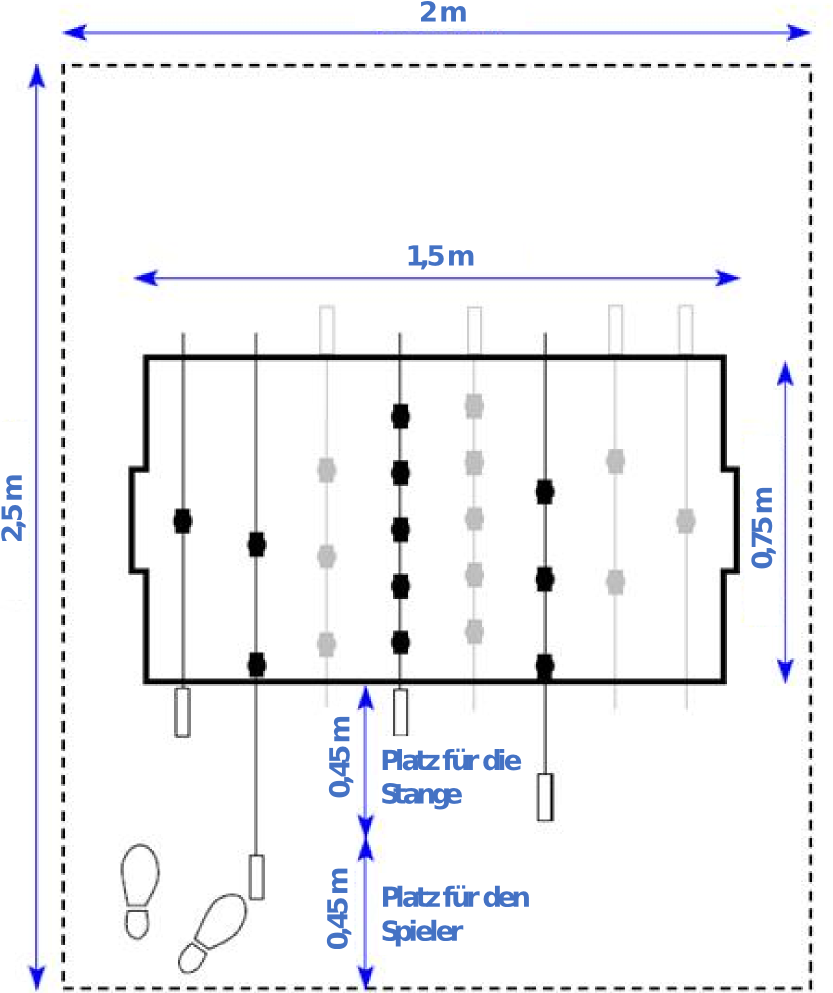
\includegraphics[width=\textwidth]{img/tisch_platzbedarf.png} 
            \caption{Platzbedarf} 
            \label{fig:tisch:platzbedarf} 
            \vspace{0.5cm}
        \end{subfigure} 
        \begin{subfigure}[b]{0.7\textwidth} 
            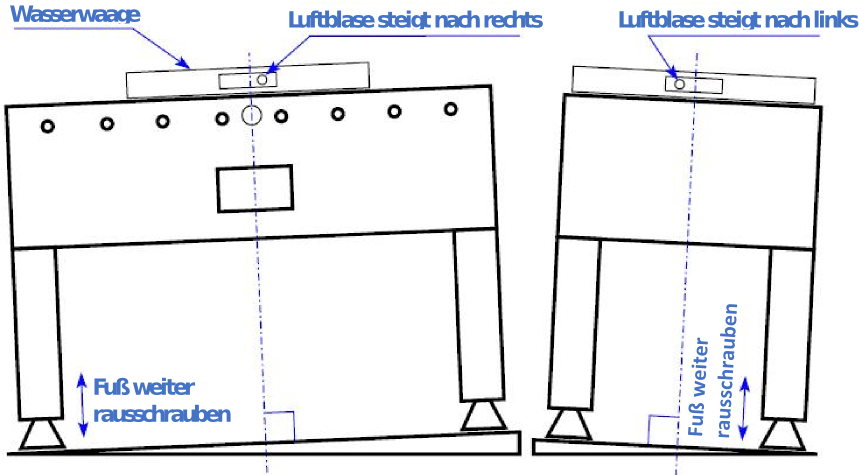
\includegraphics[width=\textwidth]{img/tisch_ausrichten.png} 
            \caption{Ausrichten} 
            \label{fig:tisch:ausrichten} 
        \end{subfigure} 
        \label{fig:tisch} 
        \caption{Aufstellen eines Tischs [\cite{itsf_basics}]} 
\end{figure}
    %\end{wrapfigure}

%%%%%%%%%%%%%%%%%%%%%%%%%%%%%%%%%%%%%%%%%%%%%%
\subsection{Pflege und Wartung}
\label{tisch:tisch:wartung}

Um einen gleichbleibenden Spielspaß zu haben, wird eine regelmäßige Tischpflege und Wartung empfohlen:
\begin{itemize}  
    \item {\normalfont \bfseries Stangen:} Damit die Stangen leicht laufen, schmieren viele Spieler die Stangen mit Pronto-Spray (Möbelpolitur) oder Silikonöl, bevor Sie Tischfußball spielen. Dabei ist in jedem Fall darauf zu achten, die ganz herausgezogene oder ganz reingeschobenene Stange außerhalb des Tisches und nie über der Spielfläche zu beschmieren. Danach sollten die Stangen hin- und hergedreht werden, während man die Stange rein- und rauszieht, damit sich das Schmiermittel gut über die Stange verteilt  und die Stangen gut in den Lagern laufen.
        Weitere Infos bei \href{http://ungeblogtkickern.blogspot.de/2014/11/wie-kann-ich-die-stangen-am-besten.html}{Ungeblogt}.

    \item {\normalfont \bfseries Spielfeld:} Auf dem Spielfeld sammelt sich über die Zeit Schmutz wie bspw. Staub, abgelöste Gummistücke von den Puffern oder auch Ballspuren. Diese lassen sich am einfachsten und schonend mit etwas Glasreiniger und Haushaltspapier entfernen -- zumindest bei Soccer-Spielflächen wie bei Leonhart- oder Ullrich-Tischen. In jedem Fall sollte man auf Spülmittel und Scheuerschwämme verzichten. 
    \item {\normalfont \bfseries Lager und Puffer:} Das Schmiermittel für die Stangen kann leider auch leicht Staub binden. Diese Masse setzt sich gerne in den Lagern über die Zeit ab. Mit einem zurechtgerollten normalen Schreib-Papier kann man die Ablagerungen durch Durchschieben der Rolle entfernen. Manchmal lohnt sich aber auch eine Grundreinigung und man baut die Figuren, Stangen und Lager aus, um die Lager ohne Stange gründlich zu reinigen. Dabei sollte man sich überlegen, ob man die Puffer ersetzt. Puffer lösen sich durch die Schmiermittel und die Belastung nach einiger Zeit auf.    
    \item {\normalfont \bfseries Allgemeines:} Natürlich sollten alle Schrauben am Tisch fest sitzen. Es lohnt sich ab und zu zu überprüfen, ob alle Schrauben noch festsitzen.  
\end{itemize}  


%%%%%%%%%%%%%%%%%%%%%%%%%%%%%%%%%%%%%%%%%%%%%%
%%%%%%%%%%%%%%%%%%%%%%%%%%%%%%%%%%%%%%%%%%%%%%
\section{Bälle}
\label{tisch:baelle}

Es gibt verschiedene Typen von Bällen, obwohl der Durchmesser typischerweise 35 mm beträgt -- manchmal auch 34 mm \citep{www:kickerbau:baelle}.
Tischfußball-Bälle unterscheiden sich vor allem in ihrer Griffigkeit und ihrem Gewicht, zudem in ihrer Farbe und auch beim Material.
Insbesondere die Griffigkeit, und damit die Oberflächenbeschaffenheit des Balls, und das Gewicht sind entscheidend für die Spieleigenschaften.  

Vorgestellt werden hier drei Bälle, die auf den Soccertischen (Leonhart, Ullrich, Lettner) üblicherweise gespielt werden und alle aus weißem Plastik sind \citep{www:tfc-reutlingen}:
\begin{itemize}
    \item Der Ullrich Ball:
        Der Ullrich Ball ist durch seine eher weiche Oberfläche der griffigste Ball unter den Soccer-Bällen. 
        Das ermöglicht eine Ballführung mit viel Kontrolle. Insbesondere beim Klemmen kann man damit den Ball an verschiedenen Punkten unter der Stange führen und spielen (siehe Kapitel \ref{technik:offensive:eine:pin}).
        % Grafik ? Foto 
        Mit einem üblichen 35 mm Durchmesser wiegt der Ball 24 g.
        Dadurch das der Ball relativ weich ist, bekommt er mit der Zeit Macken und Dellen, so dass ein langsamer Ball zum Teil nicht mehr ganz gerade rollt.
        Er ist offizieller Ball in Deutschland und mit dem DTFB- und dem P4P-Schriftzug bedruckt.
        \\
        Preis: 2,00 Euro. 
        \\
        Spieler: Ab Anfänger bis Profi
    \item Der Leonhart Ball: 
        Mit einem Durchmesser von 35 mm und einem Gewicht von etwa 27 g ist im Vergleich zu vielen Bällen relativ schwer. 
        Zusammen mit seiner harten und doch leicht griffigen Oberfläche hat er damit ruhiges und genaues Rollverhalten.
        Er ist mit dem ITSF Schriftzug bedruckt, da er offizeller ITSF Ball für den Leonhart-Tisch ist.
        \\
        Preis: 2,50 Euro. 
        \\
        Spieler: Ab Fortgeschrittene bis Profi
    \item Der Lettner Ball (Contus Avant):
        Der dritte DTFB zertifizierte Ball ist für den Lettner Tisch entwickelt.
        Er hat ein Gewicht von 27 g und einem Durchmesser von 34,9 mm.
        Der Ball hat eine harte Oberfläche, ist jedoch leicht griffig. 
        Er ist nicht so verbreitet wie der Leonhart- oder Ullrich-Ball. 
        \\
        Preis: 2,75 Euro.
        \\
        Spieler: Ab Amatuer bis Profi
\end{itemize}

Die Griffigkeit hängt nicht nur von der Art des Balls ab, sondern ist ein Zusammenspiel zwischen Figur, Ball und Spieloberfläche. 
Zum Beispiel spielt sich ein Leonhart-Ball auf einem Ullrich-Tisch eher weniger griffig.  
Und auch die offiziellen Tische -- die 5 ITSF- und 3 DTFB-Tische -- haben jeweils ihren eigenen zertifizierten Ball und dadurch unterschiedlichste Spieleigenschaften:
Der Bonzini-Ball ist orange und hart, aber auf dem Bonzini-Tisch sehr griffig. 
Im Gegensatz zum Tornado Ball, der aus roten Urethan ist, was ihn sehr hart und schwer macht -- und sehr ungriffig bzw. rutschig. 



%%%%%%%%%%%%%%%%%%%%%%%%%%%%%%%%%%%%%%%%%%%%%%
\section{Zubehör}
\label{tisch:zubehoer}

Das wichtigste Spielzubehör ist für eine gute Griffigkeit verantwortlich: \nameref{tisch:zubehoer:griffe}.
Auch auf angemessene \nameref{tisch:zubehoer:kleidung} legen Amateuer- und Profi-Spieler wert.
Zudem gibt es einige \nameref{tisch:zubehoer:training}, die für ein abwechslungsreiches und fokussiertes Trainieren sorgen können.

%%%%%%%%%%%%%%%%%%%%%%%%%%%%%%%%%%%%%%%%%%%%%%
\subsection{Griffbänder und Handschuhe}
\label{tisch:zubehoer:griffe}

Alle Spielaktionen beim Tischfußball geschehen durch die Hände der Spieler, die die Stangen über die Griffe bewegen.
Egal bei welcher \nameref{technik:haltung:griffe} und egal für welche Techniken ist eine gewisse Griffigkeit notwendig. 

Obwohl die festinstalliersierten Griffe bei den DTFB-Tischen (Leonhart, Ullrich, Lettner) aus schwarzem Gummi gurndsätzlich eine gute Griffigkeit bieten, kann sich die Griffigkeit bei längerem Spiel wegen Schwitzens verschlechtern.
Daher verwenden viele Spieler (Tennis-)Griffbänder, die sie vor dem Spielen um die Griffe wickeln. 
Griffbänder bieten zwei entscheidende Vorteile:
\begin{itemize}
    \item Schweißabsorbtion und dadurch gleichbleibende Griffigkeit
    \item besserer Griff beziehungsweise bessere Stangenkontrolle
\end{itemize}
Nach dem Spielen sollte man die Bänder wieder aufwickeln, damit die Oberfläche nicht einstaubt, und die Griffigkeit erhalten bleibt.
Manche Griffbänder kann man sogar mit in der Waschmaschine waschen, so dass diese nach längerer Benutzung wieder fast  wie neu sind. 
Griffbänder gibt es von vielen verschiedenen Herstellern und kosten etwa zwischen 0,50 und 2,50 Euro. 

\paragraph{Wie wickelt man ein Griffband auf?} Die Standardwicklung (\href{https://www.youtube.com/watch?v=KgOqDdcp4n4}{Video-Link}):
\begin{itemize}
    \item[a)] Man beginnt bei der tischnäheren Seite des Griffs und wickelt nach außen.
        Man sollte darauf achten, dass der Bandanfang durch die ersten Wicklungen fixiert wird. 
    \item[b)] Durch Drehen der Stange wickelt man das Band gleichmässig auf den Griff, wobei das Band stets etwa zur Hälfte die darunter leigende Schicht überdecken sollte.
    \item[c)] Ist das Band ganz aufgewickelt, benutzt man ein Abschlussgummi, um die letzte Wicklung zu fixieren.
\end{itemize}

Ein ebenfalls beliebtes Zubehör sind (Golf-)Handschuhe. 
Damit kann man insbesondere in Kombination mit Griffschläuchen oder -gummis, die man über den Griff zieht, eine erhöhte Griffigkeit erlangen.
Dieses Material ist bei Spielern, die mit der Abroller-Technik schießen, besonders beliebt, da man mit wenig Druck auf die Stange, dennoch eine hohe Seitwärts-Bewegung erreichen kann (siehe Kapitel \ref{technik:offensive:schiessen:pin}).  

Spieler, die Jet schießen, benutzen Material um ihre Handgelenke bzw. den Unterarm. 
Manche benutzen dafür ein verkürztes Griffband bzw. eigens dafür hergestellte Jet-Armbänder.
Dadurch soll ebenfalls eine schnelle Seitwärts-Bewegung erreicht werden, bei wenig Kraftaufwand (siehe Kapitel \ref{technik:offensive:schiessen:jet}).
Weitere Infos gibt es in \href{http://ungeblogtkickern.blogspot.de/2015/05/griffe-praparieren.html}{diesem Artikel bei Ungeblogt}.

\paragraph{Hintergrund:} Da sich die Griffe der 5 offiziellen ITSF-Tische in Dicke und Form, Material und Griffigkeit unterscheiden, wurde vor einigen Jahren ein Griffwechselsystem bei internationalen Turnieren eingeführt.
Das ermöglicht den Spielern ihren Lieblingsgriff an allen Tischen zu spielen. 


%%%%%%%%%%%%%%%%%%%%%%%%%%%%%%%%%%%%%%%%%%%%%%
\subsection{Kleidung}
\label{tisch:zubehoer:kleidung}

Nach dem ITSF-Regelwerk gibt es beim Tischfußball einen Dresscode, der Sportkleidung vorschreibt. 
Bei internationalen und nationalen Wettkämpfen tragen die Spieler Trikots mit ihrem Vereinslogo und ihrem Namen darauf. 
Neben der Teamzugehörigkeit bieten Sporttrikots eine gewisse Atmungsaktivität, die bei einem schweisstreibendem Spiel von Vorteil sind. 
Manche Spieler haben sogar ein Handtuch in Tischnähe, um Ihren Schweiss in Auszeiten abzuwischen.

Während eines Turniertages ziehen sich viele Spieler, zwischen den Spielen eine Trainingsjacke an, um nicht auszukühlen.
Bei der Hosenwahl -- ob kurz oder lang -- ist es den Spielern überlasssen, wie man sich am wohlsten fühlt. 
Bei der Schuhwahl sollte man darauf achten, dass man beim Tischfußball überwiegends steht. 
Daher wird ein wohlfühlendes Schuhbett empfohlen, wie etwa ein gut gedämpfter Laufschuh.  

%%%%%%%%%%%%%%%%%%%%%%%%%%%%%%%%%%%%%%%%%%%%%%
\subsection{Podeste}
\label{tisch:zubehoer:podeste}

%TODO


%%%%%%%%%%%%%%%%%%%%%%%%%%%%%%%%%%%%%%%%%%%%%%
\subsection{Trainingsmaterialien}
\label{tisch:zubehoer:training}

%%%%%%%%%%%%%%%%%%%%%%%%%%%%%%%%%%%%%%%%%%%%%%
\subsubsection{Stangenklemmen oder Rod-Locks}
\label{tisch:zubehoer:training:rodlock}

\begin{figure}
    %\begin{wrapfigure}{r}{0.4\textwidth} 
    \centering 
        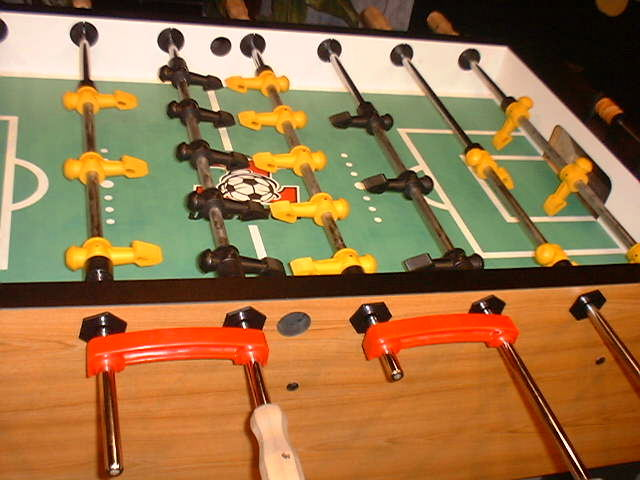
\includegraphics[width=0.38\textwidth]{img/rodlock_goalie.jpg} 
        \caption{Um ein Goalie-Einzel zu spielen, verbindet hier eine rote Stangenklemme die gelbe 3er- mit der schwarzen 5er-Reihe und eine zweite Klemme die gelbe 5er- mit der schwarzen 3er-Reihe. [\cite{www:rod-lock}]} 
        \label{fig:rod-lock} 
\end{figure}
    %\end{wrapfigure}

Stangenklemmen, oder im Englischen Rod-Locks, sind wohl das gängigsten Trainingszubehör. 
Eine Klemme kann an zwei Stellen an eine Stange geklemmt werden, so dass sich zwei Stangen miteinander fixiert werden können. 
Damit ergeben sich folgende Trainingsvarianten \citep{www:rod-lock}:
\begin{itemize}
    \item \nameref{spielformen:sonderregeln:goalie}: Mit zwei Stangenklemmen kann man die Mittelfeld- und Sturmreihen hochklappen, so dass die Spielfiguren waagrecht bleiben (siehe Abb.~\ref{fig:rod-lock}). 
        Somit kann man Torwart gegen Torwart spielen. 
        \\
        Zielgruppe: ab Anfänger
        \\
        Trainingseffekt: Torwartdasein
    \item Schusstraining: Mit einer Klemme kann man die Torwart- und 2er-Stange festklemmen. 
        Durch Variation der Distanz zwischen Torwart- und Abwehrfigur sowie deren Stellungswinkel kann man verschiedene statische Deckungen stellen.
        Dadurch kann trainieren auf verschiedene Lücken Tore zu schießen.  
        \\
        Zielgruppe: ab Fortgeschrittene
        \\
        Trainingseffekt: Hand-Auge-Koordination, Präzession beim Schiessen
    \item Mittelfeldtraining: Eine Stangenklemme and die gegnerische Mittelreihe einseitig geklemmt, so dass die Figuren nach vorne gestellt sind, wenn die Klemme nach unten hängt, ist für ein Mittelfeldtraining effektiv:
        Beim Passtraining von der 5er- auf die 3er-Stange versucht man durch die gegnerische 5er-Reihe zu spielen. 
        Trifft man die gegnerische Figur, wird der Ball durch das Auslenken der Stangenklemme automatisch zurückgespielt, so dass man zum Einen lernt die Abpraller zu kontrollieren und zum Anderen gleich den nächsten Passversuch spielen kann, ohne den Ball mit der Hand zurechtzulegen.
        \\
        Zielgruppe: ab Amateurspieler
        \\
        Trainingseffekt: Mittefeldspiel, Präzession beim Passen
\end{itemize}
Eine Stangenklemme kostet 10 bis 20 Euro -- man kann für das \nameref{spielformen:sonderregeln:goalie} jeweils zwei Stangen auch mit einem einfachen Haushaltsgummi hochstellen:
Dafür legt man den Gummi um den Kopf einer Figur (z.B. die mittlere Figur der 3er-Reihe), dreht dann das andere Ende des Gummis um eine halbe Umdrehung und legt dieses um des Kopf der Figur an der zweiten Stange (z.B. die mittlere Figur der 5er-Reihe). 

%%%%%%%%%%%%%%%%%%%%%%%%%%%%%%%%%%%%%%%%%%%%%%
\subsubsection{Weiteres Zubehör}
\label{tisch:zubehoer:training:weiteres}

\begin{itemize}
        %%%%%%%%%%%
    \item {\normalfont \bfseries Backbouncer:}
        Der Backbouncer ist aus Holz gebaute U-Form, die die Länge einer Tischbreite hat \citep{www:kickertrainer}.
        An einer Seite ist ein elastischer Zellkautschuk angebracht.
        Die U-Form lässt sich um jede Stange und deren Figuren stellen. 
        Damit prallt der Ball zurück, wenn man diesen gegen den Kautschuk schiesst: 
        Man kann alleine üben, abgeprallte Bälle zu stoppen und zu kontrollieren, in dem man verschieden stark und mit unterschiedlichen Winkeln gegen den Kautschuk spiel. 
        Den Backbouncer gibt es auch mit einem zackig geschnittenen Kautschuk, so dass der Ball unvorhergesehen abprallt.  
        \\
        Zielgruppe: ab Anfänger 
        \\
        Trainingseffekt: Hand-Auge-Koordination, Reaktion, Ballgefühl
        %%%%%%%%%%%
    \item {\normalfont \bfseries FoosTrain:}
        Mit Federn verbindet man die 2er- und die 3er-Stange \citep{www:foostrain}.
        Sobald man eine Seitwärts-Bewegung macht, folgt die Abwehrstange der Bewegung, so dass man schnell genug zum Schuss kommen muss, um nicht von der heranfahrenden Abwehrfigur gehalten zu werden.
        Durch größere Federstärken erhöht man den Schwierigkeitsgrad, da die Abwehrstange schneller der Bewegung folgt.
        \\
        Zielgruppe: ab Fortgeschrittene
        \\
        Trainingseffekt: Schusstechnik und Bewegungsablauf 
        %%%%%%%%%%%
    \item {\normalfont \bfseries Table Soccer Coach oder Visual-Kickertrainer:}
        Der Table Soccer Coach ist eine Smart-Phone App \citep{www:tablesoccercoach}:
        Man legt das Gerät über das Tor und startet das Programm. 
        Nach einer zufälligen Zeit erscheint dann ein Signal und man muss schießen.
        Neben dem akkustischen Signal gibt es noch ein visuelles Signal auf dem Display, das anzeigt, welche Lücke man schießen soll.
        Ähnlich funktioniert der Visual-Kickertrainer, der durch eine LED-Leiste realisiert ist \citep{www:visualkickertrainer}.
        \\
        Zielgruppe: ab Amateurspieler 
        \\
        Trainingseffekt: Abrufbarkeit der Schüsse, Entscheidungsgeschwindigkeit
        \\
        Weitere Infos bei \href{http://ungeblogtkickern.blogspot.de/2015/01/table-soccer-coach.html}{Ungeblogt}.

        %%%%%%%%%%%
    \item {\normalfont \bfseries Kickertrainer:}
        Der Kickertrainer ist im Prinzip ein verkürzter Tisch: Das Spielfeld ist 3 Stangen lang \citep{www:kickertrainer}. 
        Damit kann man ihn schnell auf- und abbauen und zu Hause unterbringen, falls man nicht den Platz für einen Kickertisch hat.
        Zudem kann man sich mittels Holzplättchen verschiedene Lücken stellen, durch die man Passen oder Schiessen muss. 
        \\
        Zielgruppe: ab Anfänger 
        \\
        Trainingseffekt: Präzession beim Passen und Schiessen
        %%%%%%%%%%%
    \item {\normalfont \bfseries Kicker Maschine:} 
        Die Kicker Maschine ist eine junge Entwicklung, die es noch nicht zu kaufen gibt, aber eine interessante Trainingsmöglichkeit bietet \citep{www:kickermaschine}. 
        Durch ein Motor-betriebenes Hebelsystem werden die gegnerischen Stangen automatisch hin- und herbewegt. 
        Dadurch kann man das Passen und Schiessen üben, während sich die gegnerischen Stangen rythmisch bewegen.
        \\
        Zielgruppe: ab Amateuerspieler 
        \\
        Trainingseffekt: Deckungsanalyse und Timing

\end{itemize}


%%%%%%%%%%%%%%%%%%%%%%%%%%%%%%%%%%%%%%%%%%%%%%%%%%%%%%%%%%%%%
% regeln
\chapter{Regeln}
\label{regeln}


\section{Grundlagen}
Anlehnung an ITSF Basisregeln / P4P Rookie Regeln / DTFB Grundregeln
\section{Regelfahrplan}
Schrittweise Hinführung zum ITSF Regelwerk (Einmannpass, Pass mit laufendem Ball, ...)
\section{ITSF Regelwerk}




%%%%%%%%%%%%%%%%%%%%%%%%%%%%%%%%%%%%%%%%%%%%%%%%%%%%%%%%%%%%%
% technik und taktik 
\chapter{Technik}
\label{technik}

Beim Tischfussball ist das Toreschiessen das wichtigste um zu Gewinnen und daher ist das Spiel von Anfängern durch viele schnelle (Direkt-)Schüße geprägt.
Vor allem durch Trichschüsse heben sich erfolgreichere Spieler hervor.
Im Amateur-Bereich kommen meist Pass- und Schuss-Optionen hinzu.
Und im Profi-Bereich werden meist alle Techniken angewandt, vor allem um strategisch eine Partie zu gewinnen. siehe nächstes Kapitel~\ref{taktik}. 
Bei allen Spielniveaus werden verschiedene Defensivtechniken angewandt, um die Offensive des Gegners erfolgreich zu verteidigen.
All diese Techniken sind notwendig für ein kontrolliertes Spiel -- was der eigentlich Trick der Profis ist.

Technik ist die Grundlage eines jeden Sports. 
Das Ziel einer sauberen Technik ist das Kontrollieren des Balles mit den Spielfiguren in unterschiedlichen Spielsituationen:
\begin{itemize}
    \item in der Offensive (Kapitel \ref{technik:offensive}) und bei Ballbesitz gibt es Techniken für 
        \begin{itemize}
            \item das Passen, 
            \item das Annehmen und 
            \item das Schießen des Balles
        \end{itemize}
    \item in der Defensive (Kapitel \ref{technik:defensive}) und bei Nicht-Ballbesitz gibt es Techniken für 
        \begin{itemize}
            \item das Stellungsspiel, 
            \item das Blocken und 
            \item das Fangen des Balles  
        \end{itemize}
\end{itemize}
Zunächst in Kapitel \ref{technik:haltung} wird die grundlegende Körper- und Griffhaltung beschrieben, wobei sich vor allem die Griffhaltung und Arm- und Oberkörperbewegung beim Spielen der Techniken verändern kann. 

\paragraph{Technik-Training;} 
Das Erlernen der Techniken und entprechendes Training sollte dem Spielniveau und dem Alter angepasst werden. 
Spielerisches Erlenen (siehe Kapitel~\ref{chap:spielformen}) ist etwa für Kinder und Jugendliche und Anfänger geeignet, regelmäßige Wettkämofe (Liga und Turniere) für Fortgeschrittene und statisches Techniktraining für ambitionierte Spieler.


%%%%%%%%%%%%%%%%%%%%%%%%%%%%%%%%%%%%%%%%%%%%%
\section{Körper- und Handhaltung}
\label{technik:haltung}

Bei Ballsportarten sind die Körperstellung und der Stand zum Ball eine Grundvorraussetzung zum erfolgreichen Spiel.
Bei Schlägersportarten sind die Handhaltung und die Arm- und Körperbeweglichkeit eine Grundvorraussetzung zur erfolgreichen Ausführung einer Spielaktion.
Diesen beiden Aspekte sind auch beim Tischfussball zu beachten:
Ein richtiger Stand zum Tisch beinhaltet eine eine lockere Grundbeweglichkeit von Körper und vor allem den Armen und Händen zum Bewegen der Stangen (Kapitel~\ref{technik:haltung:koerper}),
Eine richtige Handhaltung der Stangen umfasst das einer Spielsituation bedingtes Drehen und Schieben und Ziehen der Stangen und damit Spielen des Balles (Kapitel~\ref{technik:haltung:griffe}).
Die folgenden Kapitel geben eine grundlegende Richtlinie zur richtigen Haltung, die für jeden individuell anders ist. 

\begin{figure}
    \centering 
        \begin{subfigure}[b]{0.9\textwidth} 
            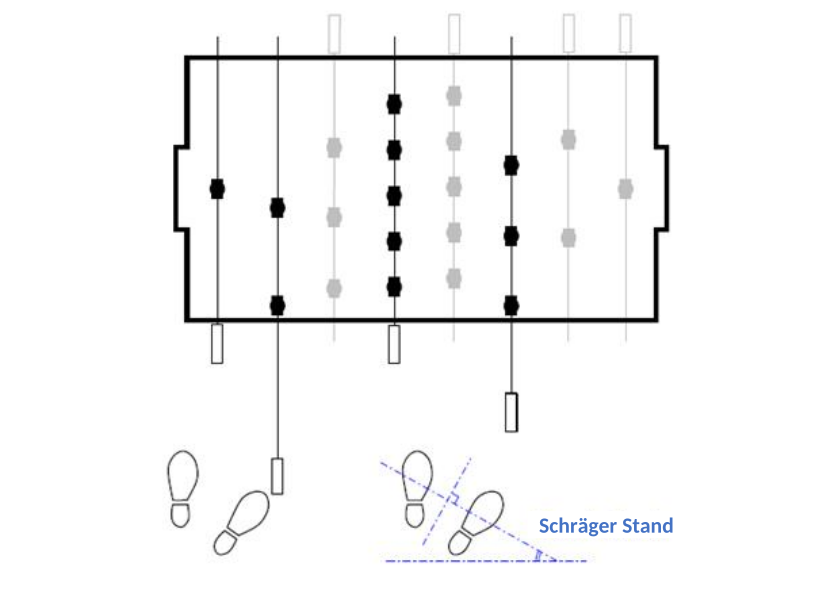
\includegraphics[width=\textwidth]{img/haltung_koerper.png} 
            \caption{Grundlegender Körperstand} 
            \label{fig:haltung:koerper} 
            \vspace{0.5cm}
        \end{subfigure} 
        \begin{subfigure}[b]{0.5\textwidth} 
            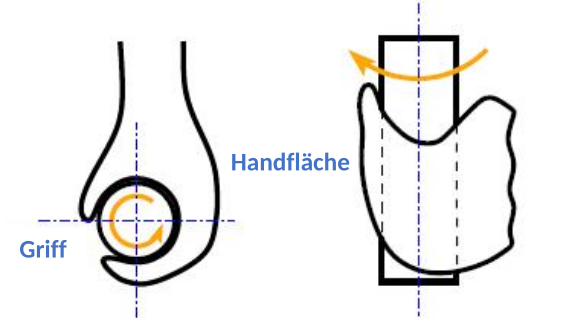
\includegraphics[width=\textwidth]{img/haltung_hand.png} 
            \caption{Grundlegende Handhaltung} 
            \label{fig:haltung:hand} 
        \end{subfigure} 
        \label{fig:haltung} 
        \caption{Die grundlegenden Haltungen [\cite{itsf_basics}]} 
\end{figure}

%%%%%%%%%%%%%%%%%%%%%%%%%%%%%%%%%%%%%%%%%%%%%
\subsection{Körperhaltung}
\label{technik:haltung:koerper}

Die Grundhaltung ist ein schulterbreiter Stand.
Der Abstand vom Körper zum Tisch mit einem leichten schrägen Stand mit Blick zum Tor (siehe Abbildung \ref{fig:haltung:koerper}) sollte so sein, dass die Stangen beweglich ganz rein- und rausgefahren und gedreht werden können.
Dabei kann der rechte Arm aus der Schulter seitlich am Körper vor und zurück bewegt werden. 

Ein lockerer Stand sollte die Arme für flüssige Stangenbewegungen entlasten. 
Daher sollte man sich etwa nicht auf den Griffen abstützen.
Hierbei hilft es leicht in die Knie zu gehen und das Körpergewicht leicht auf die Fussballen zu verlagern; der Oberkörper ist meist gebeugt zum Tisch, dabei sollte der Rücken einigermaßen gerade und die Schultern locker sein.

Diese Grundhaltung ist statisch, dass bedeutet die Füße behalten ihre Position. 
Meist wird diese statische Haltung weitestgehend bei der Ausführung eines Passes oder Schusses beibehalten. 
Leichte Positionsänderungen passieren für einen angepassten Stand etwa für eine bestimmte Schusstechnik (Zieher, Schieber, Abroller/Front-Pin) und Defensivtechniken.
Und in der Einzeldisziplin muss der Spieler sich am Tisch ständig bewegen und seine Position der jeweiligen Ballposition bzw. der gewollten Stangenkontrolle anpassen.

\paragraph{Hinweis:} Um Rückenproblemen vorzubeugen, sollte neben der entspannten Körperhaltung eine Ausgleichsbewegung vor oder nach dem Tischfussballspielen gemacht werden.
Das kann eine andere Sportart sein, aber auch schon ein paar kurze Aufwärm- und Lockerungsübungen können entspannen: Hüpfen, Armkreisen, Luftklettern, usw. 

%%%%%%%%%%%%%%%%%%%%%%%%%%%%%%%%%%%%%%%%%%%%%
\subsection{Handhaltung}
\label{technik:haltung:griffe}

Die standardmäßige Handhaltung ist eine geschlossene
und der Handrücken zeigt dabei nach oben (siehe Abbildung~\ref{fig:haltung:hand}).
Wird der Griff so gehalten, wenn gleichzeitig die Figuren mit den Füßen nach unten stehen, kann die Stange durch Bewegen des Handgelenks so gedreht werden, dass die Füße der Figuren die volle Drehbereich Abfahren (siehe Abbildung~\ref{fig:figurdrehen}):
\begin{itemize}
    \item von ganz hinten, um einen \textit{Ball hinter der Stange} zu spielen (Hinten Klemmen, Back-Pin, Brush/Drücker, Druckpunkt, Fangen, siehe Kapitel \ref{}), über
    \item gerade Figuren-Position für Tic-Tac (Kapitel \ref{}) die volle Abdeckung (Kapitel \ref{}) bis 
    \item ganz vorne, um einen \textit{Ball vor der Stange} zu spielen (Vorne Klemmen, Front-Pin, Fangen, siehe Kapitel \ref{}).
\end{itemize}

\begin{figure}
    \centering 
        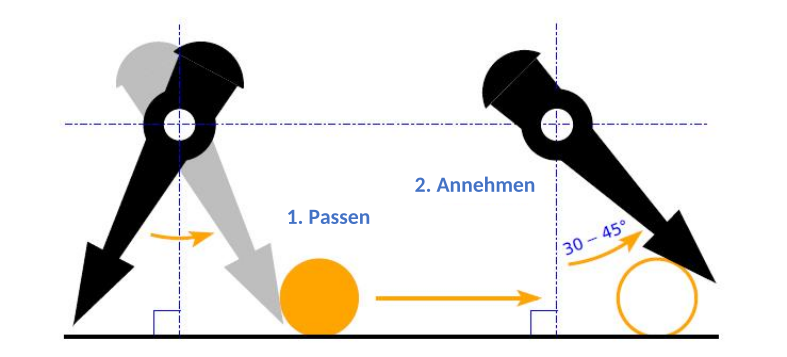
\includegraphics[width=0.7\textwidth]{img/haltung_figur.png} 
        \caption{Drehung der Stange: Verschiedene Figurpositionen, hinter der Stange (links), rechts vor der Stange (rechts) [\cite{itsf_basics}]} 
        \label{fig:haltung:figur} 
\end{figure}

Der Griff wird je nach Technik unterschiedlich stark festgehalten oder mit verschiedenen Drehgeschwindigkeiten bewegt. 
Grundsätzlich lässt  eine lockere Handhaltung die Stange in den Lagern frei und damit letztendlich schnell bewegen.
Das gilt für Seitwärts-Bewegungen der Stange und für Drehbewegungen der Stange.

Je nach Körperhaltung und Position, ist der Unterarm unterschiedlich geneigt und damit die Achse des Handgelenks unterschiedlich zur Drehachse der Stange.
Hier gibt es Anpassungen je nach Technik (Zieher, Schieber, Linke-Hand-Pass, Defensiv-Stellungen) oder nach indivueller Haltung.

Eine erste abweichende Griffhaltung ist der Fingergriff: Hierbei halten die Fingerspitzen das Griff Ende, der Unterarm ist fast waagrecht, und die Stange kann aus dem Unterarm schnell gedreht werden.
Für die Schusstechniken Abroller/Front-Pin und Jet gibt es eine komplett andere Grundhaltung des Griffs, siehe Kapitel~\ref{} bzw. \ref{}.


%%%%%%%%%%%%%%%%%%%%%%%%%%%%%%%%%%%%%%%%%%%%%
%%%%%%%%%%%%%%%%%%%%%%%%%%%%%%%%%%%%%%%%%%%%%
\section{Offensive: Passen, Annehmen, Schiessen}
\label{technik:offensive}

Beim Tischfussball ist die \gls{offensive} bei Ballbesitz möglich.
Dabei können die Figuren durch Bewegen der Stange nur im jeweiligen Bereich den Ball erreichen und spielen (vergleiche Abbildung~\ref{fig:tischbereiche}).
Ballkontrolle oder Ballgefühl beinhalten das Passen, das Annehmen und das Schiessen des Balles.



%%%%%%%%%%%%%%%%%%%%%%%%%%%%%%%%%%%%%%%%%%%%%
\subsection{Ballführung (auf einer Stange)} 
\label{technik:offensive:eine}

Figur zum Ball: Spielen und annehmen

\begin{itemize}
\item Ruhender Ball und Puppenwechsel.
\item Tictac oder Vorne-hinten Klemmen.
\item Auf der 2er-Stange zwischen der 1. und der 2. Puppe.
\item Auf der 3er-Stange zwischen der 1. und der 2. Puppe oder der 2. und der 3.Puppe oder mit der 1. und 3. Puppe.
\item Auf der 5er-Stange zwischen der zwei benachbarten Puppen oder mit zwei Puppen und dabei eine Puppe auslassen.
\end{itemize}


%%%%%%%%%%%%%%%%%%%%%%%%%%%%%%%%%%%%%%%%%%%%%
\subsection{Passen (zwischen zwei Stangen)}
\label{technik:offensive:zwei}

Figur zum Ball: Spielen und annehmen

\begin{itemize}
\item Spielprinzipien: Ins Feld, gerade oder an die Bande.
\item Passtechniken: Kanten-, Stick und Brushpass. 
\href{http://ungeblogtkickern.blogspot.de/2015/09/schrag-schieen.html}{Artikel auf Ungeblogt}
\item Annahmetechniken: Ballanahme.
\end{itemize}

Passmöglichkeiten:
\begin{itemize}
\item Von der 5er- auf die 3er-Stange.
\item Von der 2er-Stange auf die 3er-Stange.
\item Von der 2er-Stange auf die 5er-Stange.
\end{itemize}


%%%%%%%%%%%%%%%%%%%%%%%%%%%%%%%%%%%%%%%%%%%%%
\subsection{Torschüsse}
\label{technik:offensive:torschuesse}

\begin{itemize}
\item Schussprinzipien: Schneller als der Gegner, Seitwärtsbewegung und Schussbewegung. Für Fortgeschrittene: Geschwindigkeit, Präzision, Konstanz, Abrufbarkeit
\item Schusstechniken: Schieber/Zieher, \href{http://ungeblogtkickern.blogspot.de/2014/07/schritt-fur-schritt-pin-schieen.html}{Abroller/Pin} oder Jet.
\item Von der 3er-Stange oder der 2er-Reihe.
\item Trickschüsse
\end{itemize}





%%%%%%%%%%%%%%%%%%%%%%%%%%%%%%%%%%%%%%%%%%%%%
%%%%%%%%%%%%%%%%%%%%%%%%%%%%%%%%%%%%%%%%%%%%%
\section{Defensive: Stellen, Blocken, Fangen}
\label{technik:defensive}

\begin{itemize}
\item Defensiv-Prinzip: mit den Figuren die direkten Ballwege zum Tor blockieren (Seitwärtsbewegung)  
\item Klapprichtung der Figuren und Abstand der Figuren (Drehbewegung)
\item Bälle blocken, fangen, annehmen 
\end{itemize}
Daraus folgen grundlegende sogenannte Stellungsspiele.


\subsection{Ballbesitz des Gegners im Abwehrbereich}
\label{technik:defensive:gegnerabwehr}

\begin{itemize}
\item Deckung als Stürmer
\item Deckung als Torwart: (statisch) im kurzen/langen Eck
\item Deckung im Doppel
\item Deckung im Einzel
\end{itemize}


\subsection{Ballbesitz des Gegners im Mittelfeld (5er-Reihe)}
\label{technik:defensive:gegnermittelfeld}

\begin{itemize}
\item Deckung als Stürmer (5er-Reihe): Pass verhindern, kleinster Fahrbereich, an die Bande fahren
\item Deckung als Torwart: Torschüße, direkter Ballweg
\end{itemize}


\subsection{Ballbesitz des Gegners im Sturm (3er-Reihe)}
\label{technik:defensive:gegnersturm}

\begin{itemize}
\item Deckung als Torwart: Reaktion, fahren, shaken, Wechseln
\end{itemize}



%%%%%%%%%%%%%%%%%%%%%%%%%%%%%%%%%%%%%%%%%%%%%%%%%%%%%%%%%%%%%
% systemspiel 
\chapter{Systemspiel (Taktik)}
\label{taktik}

\section{Motivation: Strategien zu Gewinnen.}

Schussprinzipien: Schneller als der Gegner, Seitwärtsbewegung und Schussbewegung. Für Fortgeschrittene: Geschwindigkeit, Präzision, Konstanz, Abrufbarkeit

\section{Offensive -- mit Ball}

\subsection{Abwehr (Torwart und 2er Reihe)}
\label{taktik:offensive:abwehr}

\begin{itemize}
    \item Torschüsse und Pässe auf den Sturm 
    \item mehrere Optionen von einem Punkt aus
\end{itemize}

\subsubsection{Zieher}
Schräges System

\subsubsection{Pin}
\href{http://ungeblogtkickern.blogspot.de/2014/12/schusssystem-linkslang-pin-aus-der.html}{Gerades System}
(Besser wäre Rechtslang Pin)

\subsubsection{Banden}
Von Mittelpunkt



\subsection{Sturm (3er Reihe)}
\label{taktik:offensive:sturm}

Torschüsse, Duell gegen den Torwart.

\begin{itemize}
    \item \href{http://ungeblogtkickern.blogspot.de/2015/11/3-punkte-theorie-auf-der-3er-reihe.html}{3 Punkte Theorie (Lücken)}
    \item Mittel-Systeme
    \item Lang-Systeme
    \item (Drei)Viertel-Systeme
    \item Systemunterschiede (Welches System das richtige für mich?)
\end{itemize}

\subsubsection{Jet Mitte}
\href{http://ungeblogtkickern.blogspot.de/2015/06/system-jet-mitte.htmli}{
    Statisches Mittesystem}
\subsubsection{Pin Mitte}
\href{http://ungeblogtkickern.blogspot.de/2015/08/system-pin-mitte.html}{
    Dynamisches Mittesystem}
\subsubsection{Pin Rechtslang}
\href{http://ungeblogtkickern.blogspot.de/2015/07/system-pin-rechtslang.html}{
    Langes Langsystem}

\begin{figure}
    %\begin{wrapfigure}{r}{0.4\textwidth} 
    \centering 
        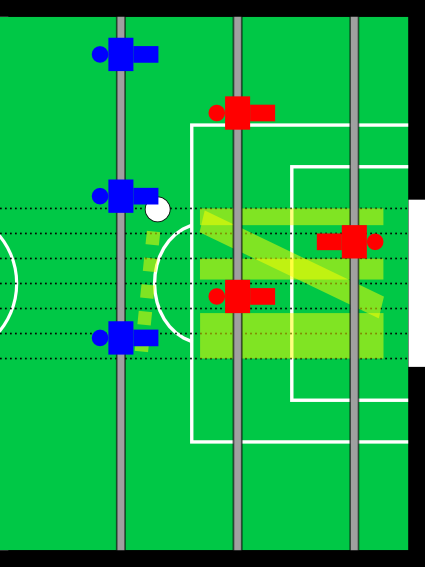
\includegraphics[width=0.25\textwidth]{img/schuss3er_lang.png} 
        \caption{Rechtslang} 
        \label{fig:rechtslang} 
    \end{figure}
    %\end{wrapfigure}

\subsubsection{Jet Linkslang}
\href{http://ungeblogtkickern.blogspot.de/2015/07/system-jet-linkslang.html}{
    Kurzes Langsystem}
\subsubsection{Zieher}
\href{http://ungeblogtkickern.blogspot.de/2015/09/system-zieher.html}{
    Statisches, schräges Langsystem}


\subsection{Passen und Schiessen (5er Reihe)}
\label{taktik:offensive:passen}

\begin{itemize}
    \item \href{http://ungeblogtkickern.blogspot.de/2015/11/passspiel-1-passeigenschaften.html}{2 Punkte Theorie und Passeigenschaften}
    \item \href{http://ungeblogtkickern.blogspot.de/2015/11/passspiel-2-setup.html}{Anrollen}
    \item Mittelfeldschüsse 
\end{itemize}


\section{Defensive -- ohne Ball}
\label{taktik:defensive}

Grundsätzliches
\begin{itemize}
    \item Den Ball erobern für Ballbesitz und eigene Offensivaktionen. Mit den Figuren die direkten Ballwege zum Tor blockieren und den Ball annehmen/fangen. 
    \item Antizipieren: Was kann passieren? Gegner lesen: Was hat der Gegner vor? (Spielart, Spielniveau, Lieblingsschuss, Entscheidung, ...)
\end{itemize}

Strategien:
,,Re-aktion'': Auf den Ball reagieren, also die Laufbahn des Balls mitverfolgen oder ,,Aktion'':
\begin{itemize}
    \item Locken (Lücke)
    \item Erschweren (Shuffle)
    \item Kreuzen (Wegziehen)
    \item Außenmann 
    \item \href{http://ungeblogtkickern.blogspot.de/2015/06/defensivbewegungen-im-verteidigerbereich.html}{Artikel auf Ungeblogt}
\end{itemize}


\subsection{Abwehr: Torwart- und 2er-Reihe}
\label{taktik:defensive:halten}

3 Punkte Deckung


\subsection{Mittelfeld (5er-Block)}
\label{taktik:defensive:5erblock}

\begin{itemize}
    \item Locken (Lücke)
    \item Erschweren (Shuffle)
    \item Zurückfahren (Wegziehen)
\begin{itemize}
    \item \href{http://ungeblogtkickern.blogspot.de/2015/05/5er-defensive.html}{Grundlagen 1}
    \item \href{http://ungeblogtkickern.blogspot.de/2015/06/defensivbewegungen-auf-der-5er-reihe.html}{Grundlagen 2}
\end{itemize}  
\end{itemize}  

\subsection{Aktives Stellungsspiel}
\label{taktik:defensive:aktivesstellungsspiel}

\begin{itemize}
    \item Aufbau an der 5er Reihe
    \item Schräge Systeme
    \item Gerade Systeme
    \item Wechsel zwischen verschiedenen Systemen
    \item Runterklappen Sturm und Mittelfeld
\end{itemize}


%%%%%%%%%%%%%%%%%%%%%%%%%%%%%%%%%%%%%%%%%%%%%%%%%%%%%%%%%%%%%
% mentales spiel und spielpsychologie 
\chapter{Spielpsychologie}
\label{psychologie}

\section{Grundlagen}
Spaß haben, Tricks zeigen, ausprobieren und natürlich Tore schießen 

Gewinnen, Verlieren und auf das nächste Mal freuen 



\section{Fortgeschrittene}
nicht für die Grundlagen

\subsection{Kontrolliert}
Zeitlassen bei Aktionen und Timeouts, Quote, Überlegenheit, nicht beinflussen
\subsection{Arbeiten}
Aktive Stangenbewegung, mehr Risiko, schnelle Überraschungsaktionen, den Gegner unter Druck setzen

\section{Profi}
nicht für die Grundlagen


%%%%%%%%%%%%%%%%%%%%%%%%%%%%%%%%%%%%%%%%%%%%%%%%%%%%%%%%%%%%%
% spielformen
%%%%%%%%%%%%%%%%%%%%%%%%%%%%%%%%%%%%%%%
\chapter{Spielformen und Trainingsspiele}
\label{spielformen}

Im Tischfußball gibt es Wettkämpfe für drei Disziplinen: 
\begin{itemize}
\item \nameref{spielformen:npersonen:einzel}
\item \nameref{spielformen:npersonen:doppel}
\item \nameref{spielformen:npersonen:team}
\end{itemize}
Neben diesen Grundspielformen gibt Varianten, die zum Training da sind und Spaß machen. Dabei wird in drei Bereichen unterteilt:
\begin{itemize}
\item \nameref{spielformen:zaehlweisen}
\item \nameref{spielformen:npersonen}
\item \nameref{spielformen:sonderregeln}
\end{itemize}
Die jeweiligen Spielformen werden in diesem Kapitel vorgestellt. Darüberhinaus kann man sich neue Varianten ausdenken, in dem man Spielformen der drei Bereiche kombiniert: Man legt fest, wie man zählt, mit wie vielen Personen man spielt und mit welchen etwaigen Sonderregeln.

\paragraph{Didaktischer Hintergrund:} Diese Variationen bieten sich insbesondere für das sogenannte {\it  genetische Lernen} in Gruppen an: Nach dem Spielen einer Spielform wird gemeinsam reflektiert, was gut war und wo der Spaß eventuell zu kurz kam. Gemeinsam wird diskutiert, welche Sonderregeln und Spielformen beim naechsten Mal festgelegt werden, um den Spaß in der Gruppe hoch zu halten und das spielerische Lernen attraktiv zu machen. 

%%%%%%%%%%%%%%%%%%%%%%%%%%%%%%%%%%%%%%%
%%%%%%%%%%%%%%%%%%%%%%%%%%%%%%%%%%%%%%%
\section{Zählweisen}
\label{spielformen:zaehlweisen}

Beim Tischfußball muss man Tore schießen und am besten mehr als sein Gegenspieler, um am Ende zu gewinnen.
Es gibt jedoch verschiedene Zählweisen, auf die man sich vor Beginn des Spiels einigt oder die bei Turnieren gespielt werden. 

%%%%%%%%%%%%%%%%%%%%%%%%%%%%%%%%%%%%%%%
\subsection{Ein Satz}
\label{spielformen:zaehlweisen:einsatz}

Wenn man einfach so kickert ohne ein Turnier zu spielen, spielt man oft einen Satz bis 6 Tore: Wer zuerst 6 Tore geschossen hat, gewinnt die Partie.
Als wichtigste Variante gilt die Unentschiedenregel: Bei 5 zu 5 Toren geht der Satz unentschieden aus.

\paragraph{Hintergrund:}
Obwohl bei vielen Tischmodellen die Torzähler 10 Tore zählen können, wird meistens bis 6 Tore gespielt -- aber auch ein Satz bis 5 oder 7 Toren sind verbreitet.
Spiele, die über einen Satz gehen, werden bei Turnieren oft in der Vorrunde gespielt.


%%%%%%%%%%%%%%%%%%%%%%%%%%%%%%%%%%%%%%%
\subsection{Mehrere Gewinnsätze}
\label{spielformen:zaehlweisen:gewinnsaetze}

Wie beim Tennis, spielt man bei Tischfußballpartien über mehrere Gewinnsätze -- das heißt, wer zuerst eine festgelegte Anzahl von Sätzen gewinnt, gewinnt die Partie. Am gängigsten sind:
\begin{itemize}
\item Zwei Gewinnsätze (engl. "Best of three"): Derjenige, der zuerst zwei Sätze gewinnt, gewinnt die Partie. Mit 2:0 Sätzen hat man also gewonnen. 
Es können maximal drei Sätze gespielt werden: Falls es nach den ersten beiden Sätzen 1:1 steht, gibt es einen dritten entscheidenden Satz, und die Partie geht 1:2 oder 2:1 aus. 
\item Drei Gewinnsätze (engl. "Best of five"): Derjenige, der zuerst drei Sätze gewinnt, gewinnt die Partie, beispielsweise 3:1. Steht es 2:2 nach den ersten vier Sätzen, gibt es einen fünften und entscheidenden Satz. 
\end{itemize}
Die Sätze werden hier jeweils bis 5 Tore gespielt. Kommt es zu einem Entscheidungsatz, also in Satz 3 bei zwei Gewinnsätzen oder in Satz 5 bei drei Gewinnsätzen, gibt es eine Verlängerung, wenn es 4:4 Tore steht: Jetzt braucht man zwei Tore Vorsprung, um den letzten Satz und damit die Partie zu gewinnen. Bei drei Gewinnsätzen kann eine sehr knappe Partie zum Beispiel 4:5, 5:4, 4:5, 5:4 und 8:6 in Toren und damit 3:2 in Sätzen ausgeht. 

\paragraph{Hintergrund:}
Mehrere Gewinnsätze werden oft bei Turnieren in der KO-Runde gespielt. Hierbei setzt sich am Ende meist das bessere Team durch. 
Und: Bei manchen Tischmodellen sind extra Satzzähler neben den Torzählern angebracht. 




%%%%%%%%%%%%%%%%%%%%%%%%%%%%%%%%%%%%%%%
%%%%%%%%%%%%%%%%%%%%%%%%%%%%%%%%%%%%%%%
\section{Anzahl der Spieler}
\label{spielformen:npersonen}

Tischfußball kann man mit unterschiedlich vielen Spielern spielen. 
Neben den drei Grundspielformen 
\begin{itemize}
\item \nameref{spielformen:npersonen:einzel},
\item \nameref{spielformen:npersonen:doppel} und 
\item \nameref{spielformen:npersonen:team}, 
\end{itemize}
gibt es auch die Möglichkeit mit drei, fünf, sechs, sieben, acht oder sogar mehr Personen an einem Tisch zu kickern.
Hierbei wird ansonsten nach den normalen \nameref{regeln} gespielt.

Hat man einen Spielmodus gewählt, kann man damit ein Training oder \nameref{turniere} gestalten, sodass möglichst alle Teilnehmer viele Spiele machen können. 


%%%%%%%%%%%%%%%%%%%%%%%%%%%%%%%%%%%%%%%
\subsection{Einzel}
\label{spielformen:npersonen:einzel}

\begin{itemize}
\item Spieleranzahl: 2
\item Aufstellung: Eins gegen eins; jeder bedient mit seinen zwei Händen seine vier Stangen.
%\item Regeln: Normale \nameref{regeln} 
\item {\bf Hintergrund:} Nur in der Einzel-Disziplin, der Doppel-Disziplin und der Team-Disziplin werden Titel vergeben: Landesmeister, Deutscher Meister und Weltmeister!  
\end{itemize}
 
%%%%%%%%%%%%%%%%%%%%%%%%%%%%%%%%%%%%%%%
\subsection{Doppel}
\label{spielformen:npersonen:doppel}

\begin{itemize}
\item Spieleranzahl: 4
\item Aufstellung: Zwei gegen zwei; jedes Team hat einen Torwart, der die 1er- und 2er-Stange bedient, und einem Stürmer, der die 5er- und 3er-Stange bedient.
%\item Regeln: Normale  \nameref{regeln} 
\item {\bf Hintergrund:} Es ist nicht klar, welches die Königsdisziplin im Tischfußball ist: Einzel oder Doppel? Fest steht das gute Einzelspieler auch gute Doppelspieler sind und anders herum -- und auch gute Teamspieler: 
Bei den Weltmeisterschaften werden die Einzelweltmeister am Freitag, die Doppelweltmeister am Samstag und am Sonntag als Letztes und als Höhepunkt die Teamweltmeister ausgespielt. 
\end{itemize}

%%%%%%%%%%%%%%%%%%%%%%%%%%%%%%%%%%%%%%%
\subsection{Team}
\label{spielformen:npersonen:team}

\begin{itemize}
\item Spieleranzahl: 2mal mindestens 3 Spieler
\item Spielplan: Es gibt einen Spielplan mit Einzel- und Doppelpartien, die typerweise auf einen Satz mit Unentschieden. Zum Beispiel:
\begin{itemize}
\item Teamgröße: Jedes Team hat jeweils drei Spieler
\item Spielmodus: Es werden 6 Spiele gespielt, nämlich drei Einzel und drei Doppel im Wechsel: Einzel 1, Doppel 1, Einzel 2, Doppel 2, Einzel 3 und Doppel 3.
\item Aufstellung: Jeder spielt ein Einzel und zwei Doppel mit dem jeweils anderen, also in Doppel 1 spielen Einzel 2 und Einzel 3 Spieler zusammen, in Doppel 2 spielen Einzel 3 und Einzel 1 Spieler und in Doppel 3 spielen Einzel 1 und Einzel 2 zusammen.  
\item Ergebnis: Gewinnt man ein Spiel bekommt man 2:0 Punkte, bei Unentschieden gibt es 1:1 Punkte, und bei einer Niederlage 0:2 Punkte. Damit sind bei 6 Spielen insgesamt 12 Punkte zu vergeben. Eine Partie kann also z.B. 12:0 oder 7:5 oder 6:6 ausgehen. 
\end{itemize}
%\item Regeln: Normale Regeln 
\item Varianten: Je nach Teamgröße kann man den Spielplan und die Aufstellungsregeln variieren. 
\item {\bf Hintergrund:} Bei der Team-Weltmeisterschaft werden zum Beispiel 4 Doppel und 2 Einzel gespielt und jeder Spieler darf maximal 1 Einzel und 1 Doppel spielen. Darum muss das Team aus mindestens 8 Spielern bestehen. 
\end{itemize}

%%%%%%%%%%%%%%%%%%%%%%%%%%%%%%%%%%%%%%%
\subsection{Kleine Runde (6 Personen)}
\label{spielformen:npersonen:kleine}

\begin{itemize}
\item Spieleranzahl: 6
\item Aufstellung: Jedes Team hat jeweils drei Spieler. Jeweils eine Doppelkombination spielt einen Ball, nach einem Tor rotiert jedes Team: Der Pausierende wird Torwart, der Torwart wird Stürmer und der Stürmer pausiert den nächsten Ball, usw.
\item Trainingseffekt: Konzentration auf ein Ball und eine Position, Zusammenspiel, Spaß, Teambuilding
\item Variation: Zu fünft kann man alternativ ein festes Doppel (2 Spieler) gegen eine rotierendes 3er-Team spielen.
\end{itemize}

%%%%%%%%%%%%%%%%%%%%%%%%%%%%%%%%%%%%%%%
\subsection{Vier gegen vier}
\label{spielformen:npersonen:viergegenvier}

\begin{itemize}
\item Spieleranzahl: 8
\item Aufstellung: Jeder greift mit einer Hand eine Stange.
Wenn ein Team ein Tor erzielt, wechselt dieses die Positionen: Jeder rückt
eine Stange vor und der Stürmer geht an die Torwartstange.
\item Trainingseffekt: Konzentration auf eine Hand, Zusammenspiel, Spaß
\item Variation: Alle nur die rechte Hand, oder nur die linke Hand
\end{itemize}

%%%%%%%%%%%%%%%%%%%%%%%%%%%%%%%%%%%%%%%
\subsection{Drei gegen drei (6 Personen)}
\label{spielformen:npersonen:dreigegendrei}

\begin{itemize}
\item Spieleranzahl: 6
\item Aufstellung: Jeder greift mit einer Hand eine Stange.
Innerhalb eines Teams darf die freie Stange durch Umgreifen aktiviert werden, allerdings
dürfen sich die Hände nicht überkreuzen.
Wenn ein Team ein Tor erzielt, wechselt dieses die Positionen: Jeder rückt
eine Stange vor und der Stürmer geht an die Torwartstange.
\item Trainingseffekt: Konzentration auf eine Hand mit mehreren Stangen, Zusammenspiel, Spaß
\item Variation: Alle nur die rechte Hand, oder nur die linke Hand. 
\end{itemize}

%%%%%%%%%%%%%%%%%%%%%%%%%%%%%%%%%%%%%%
\subsection{Zwei gegen eins}
\label{spielformen:npersonen:jedergegenjeden}

\begin{itemize}
\item Spieleranzahl:  3
\item Aufstellung: Ein Doppel (Torwart- und Stürmerposition) gegen ein Einzel, wobei die Spieler die Position während des Spiels wechseln.
Jeder sammelt für sich Punkte. Man erhält einen Punkt, wenn man in der
Einzelposition ein Tor schießt und dabei bleibt jeder bei seiner Position. 
Schießt das
aktuelle Doppelteam ein Tor, wird der Stürmer zum Einzelspieler, der Torwart zum
Stürmer, und der Einzelspieler zum Torwart („gegen den Uhrzeigersinn“).
\item Trainingseffekt: Einzeltraining, Passmöglichkeiten beim Doppel, schnelles Spiel
\end{itemize}


%%%%%%%%%%%%%%%%%%%%%%%%%%%%%%%%%%%%%%
\subsection{Runde (4 und mehr Personen)}
\label{spielformen:npersonen:runde}
\begin{itemize}
\item Spieleranzahl: 4 und am Besten mehr 
\item Aufstellung: Jeder hat eine Position, die restlichen Spieler verteilen sich auf beide Tischseiten und stellen sich hinter den Stürmer an: es wird gegen den Uhrzeigersinn gewechsel.
Gespielt wird normal bis ein Tor, danach verändern sich die Postionen:
\begin{itemize}
\item Beim Team, welches das Tor kassiert: Der Torwart fliegt raus, der Stürmer
wird Torwart, der nächste in der Schlange wird Stürmer.
\item Beim Team, welches das Tor schießt: Der Torschütze ist „gerettet“ und stellt
sich auf der anderen Seite hinten an. Schießt der Stürmer das Tor, wird der
nächste in der Reihe Stürmer und der Torwart bleibt. Schießt der Torwart
das Tor (oder fällt ein Eigentor oder ein nicht eindeutiges Tor), wird der
Stürmer Torwart, und der nächste in der Reihe Stürmer.
\item Es wird solange gespielt, bis nur noch zwei im Spiel sind. Diese spielen ein Einzel, bei dem derjenige eine Krone gewinnt, der zuerst 2 Tore schießt.
\end{itemize}
\item Trainingseffekt: Zusammenspiel, Spaß, Variation
\item Variation: jeder nur eine Stange, dann braucht man mehr als 8 Spieler
\end{itemize}


%%%%%%%%%%%%%%%%%%%%%%%%%%%%%%%%%%%%%%%
\subsection{Alleine am Tisch}
\label{spielformen:npersonen:alleine}

Wenn man mal alleine am Tisch steht, kann man sich auch selbst fordern, und eine Serie von 10 Versuchen spielen: Wie viele erfolgreiche Versuche schaffe?
Hier kann sich viele Serien ausdenken:
\begin{itemize}
\item Torschüsse: 
\begin{itemize}
\item Schieber, Zieher, Abroller oder Jet.
\item Von der 3er-Stange oder der 2er-Reihe.
\item Rechts- oder Linksschuss.
\item Kurze oder lange Schüsse.
\item Trickschüsse
\end{itemize}
\item Passen:
\begin{itemize}
\item Ins Feld, gerade oder an die Bande.
\item Kanten- oder Brushpass.
\item Von der 5er- auf die 3er-Stange.
\item Von der 2er-Stange auf die 3er-Stange.
\item Von der 2er-Stange auf die 5er-Stange.
\end{itemize}
\item Ballführung: 
\begin{itemize}
\item Ruhender Ball und Puppenwechsel.
\item Tictac oder Vorne-hinten Klemmen.
\item Auf der 2er-Stange zwischen der 1. und der 2. Puppe.
\item Auf der 3er-Stange zwischen der 1. und der 2. Puppe oder der 2. und der 3.Puppe oder mit der 1. und 3. Puppe.
\item Auf der 5er-Stange zwischen der zwei benachbarten Puppen oder mit zwei Puppen und dabei eine Puppe auslassen.
\end{itemize}
\end{itemize}
Hier kann man natürlich die Sicherheit, die Schnelligkeit und Schuss- und Passhärte mit Übung gezielt steigern.


%%%%%%%%%%%%%%%%%%%%%%%%%%%%%%%%%%%%%%%%
%%%%%%%%%%%%%%%%%%%%%%%%%%%%%%%%%%%%%%%%
%%%%%%%%%%%%%%%%%%%%%%%%%%%%%%%%%%%%%%%%
\section{Sonderregeln}
\label{spielformen:sonderregeln}

Hier findet ihr eine Sammlung an Spielarten, bei denen die normalen Regeln durch Sonderregeln ergänzt werden. 
Dadurch lernt man mit Spaß und spielerisch bestimmte Trainingsinhalte, da die Sonderregeln einen bestimmte Fokus setzen. 

%%%%%%%%%%%%%%%%%%%%%%%%%%%%%%%%%%%%%%%%
\subsection{Goalie-Einzel}
\label{spielformen:sonderregeln:goalie}

\begin{itemize}
\item Niveau: ab Anfänger
\item Spieleranzahl: 2
\item Aufstellung: 3er und 5er Stangen werden hochgeklappt und mit Rodlocks oder Haushaltsgummis fixiert (siehe auch \nameref{tisch:zubehoer:training}); ein Ball.
\item Regeln: Normale Regeln plus Sonderregel des Torwartbereichs: 
  \begin{itemize}
  \item Anstoß im Torwartbereich (siehe \nameref{spielformen:sonderregeln:abstoss}).
  \item Sobald der Ball den Torwartbereich verläßt und z.B. im mittleren Spielfeldbereich unerreichbar liegen bleibt, bekommt der Gegner den Ball und bringt den Ball neu ins Spiel.
  \item Springt der Ball aus dem Tisch, bekommt wie gewohnt derjenigen den Ball, der nicht rausgeschossen hat. 
  \end{itemize}
\item Trainingseffekt: defensive und offensive Grundlagen; Torwartdasein, wie Stellungsspiel, Ball stoppen und behalten; Ballführung und Spielfeldverständnis
%\item Variationen: \nameref{spielformen:sonderregeln:mehrerebaelle}, \nameref{spielformen:sonderregeln:unterschiedlichebaelle}, \nameref{spielformen:sonderregeln:onetouch}, \nameref{spielformen:sonderregeln:speedball}
\item Info: Goalie-Einzel wird bei vielen großen Turnieren als Nebendisziplin angeboten. Also selbst die Profis haben viel Spaß bei dieser Spielform.
\end{itemize}


%%%%%%%%%%%%%%%%%%%%%%%%%%%%%%%%%%%%%%%%
\subsection{Abstoß}
\label{spielformen:sonderregeln:abstoss}

\begin{itemize}
\item Niveau: ab Anfänger
\item Spieleranzahl und Aufstellung: variabel 
\item Regeln: Normale Regeln, aber der Anstoß nach einem Tor wird im Torwartbereich ausgeführt. 
\item Trainingseffekt: Vereinfachen des Spiels durch Weglassen des Anstosses auf der 5er-Reihe; mehr Spielanteile für den Torwart, wodurch das offensive Torwartspielen  gefördert wird
%\item Variationen: \nameref{spielformen:sonderregeln:dreigegendrei}, \nameref{spielformen:sonderregeln:unterschiedlichebaelle}, \nameref{spielformen:sonderregeln:onetouch}, \nameref{spielformen:sonderregeln:speedball}
\end{itemize}

%%%%%%%%%%%%%%%%%%%%%%%%%%%%%%%%%%%%%%%%
\subsection{Mehrere Bälle}
\label{spielformen:sonderregeln:mehrerebaelle}

\begin{itemize}
\item Niveau: ab Anfänger
\item Spieleranzahl und Aufstellung: variabel, mehrere Bälle 
\item Regeln: Normale Regeln; beim Anstoß werden mehrere Bälle ins Spiel gebracht, z.B. 10 Bälle im Mittelfeld oder auf Los jeder Spieler in einer Spielfeldecke. Oder auch mit 2 (Rollerball) oder mit 3 Bällen (3-ball Rollerball), siehe unten. 
\item Trainingseffekt: Reaktion, peripheres Sehen, Spielstrategie, spielerisch fokusiertes Spiel 
%\item Variationen: \nameref{spielformen:sonderregeln:dreigegendrei}, \nameref{spielformen:sonderregeln:unterschiedlichebaelle}, \nameref{spielformen:sonderregeln:onetouch}, \nameref{spielformen:sonderregeln:speedball}
\end{itemize}


\paragraph{Rollerball}
\begin{itemize}
\item Niveau: ab Anfänger
\item Spieleranzahl und Aufstellung: 4 Spieler im Doppel, zwei Bälle.
\item Regeln: Jedes Team wirft auf Los ein Ball ein. Wenn ein Team ein Tor schießt, darf es bei Ballbesitz des zweiten Balls, das Spiel stoppen und einen Punkt/Tor zählen. 
Oder es entscheidet auf Weiterspielen: Wenn ein Team damit sein zweites Tor schießt, bekommt es zwei Punkte; 
wenn das andere Team ausgleicht, gibt es für keinen einen Punkt. Man darf einen Ball nur 3 Sekunden ruhend stoppen und maximal 10 Sekunden auf einer Stange halten. 
Wenn ein Ball raus fliegt, gibt es Neuauflage für beide Bälle, wenn der andere Ball noch im Spiel ist; sonst wird er nach normalen Regeln wieder ins Spiel gebracht. 
Wenn ein Ball unerreichbar liegen bleibt, bleibt er dort dann solange bis er angeschossen wird, oder er wird nach normalen Regeln wieder ins Spiel gebracht, falls der zweite Ball aus dem Spiel ist (Tor, aus dem Spielfeld, ...). Sonst normale Regeln.
\end{itemize}


\paragraph{Three-Ball Rollerball}
\begin{itemize}
\item Niveau: ab Anfänger
\item Spieleranzahl und Aufstellung: 4 Spieler im Doppel, drei Bälle.
\item Regeln: Normale Regeln und Rollerballregeln, siehe oben. Zum Anstoß werden alle drei Bälle eingeworfen. 
Schießt eine Team 2 Tore und das andere 1 Tor, dann gibt es 1:0 Punkte. 
Schießt ein Team sogar alle 3 Bälle ins Tor gibt es 2:0 Punkte.
\end{itemize}


%%%%%%%%%%%%%%%%%%%%%%%%%%%%%%%%%%%%%%%%
\subsection{Unterschiedliche Bälle}
\label{spielformen:sonderregeln:unterschiedlichebaelle}

\begin{itemize}
\item Niveau: ab Anfänger
\item Spieleranzahl und Aufstellung: variabel
\item Regeln: Normale Regeln, jedoch sind in den Toren unterschiedlich griffige Bälle, die nach Torerfolg zufällig ins Spiel kommen.
\item Trainingseffekt: Ballgefühl 
\end{itemize}


%%%%%%%%%%%%%%%%%%%%%%%%%%%%%%%%%%%%%%%%
\subsection{Elfmeterschießen}
\label{spielformen:sonderregeln:elfmeter}

\begin{itemize}
\item Niveau: ab Anfänger
\item Spieleranzahl: 2
\item Regeln: Es wird abwechselnd von der Stürmerreihe geschoßen (Schütze) und mit Torwart- und 2er-Stange gehalten (Torwart). Als Stürmer bringt man den Ball auf der Stürmerreihe ins Spiel und darf den Ball maximal 15 Sekunden halten, bis zu einem Schuß aufs Tor. Vor dem Schuß darf der Ball beliebig zwischen den 3 Stürmerfiguren hin und her gespielt werdne oder auch ruhen. 
Nach dem Schuß wird gewechselt und der Torwart wird Stürmer und der Stürmer Torwart.
\item Trainingseffekt: fokussierter Schuss auf der Stürmerreihe, Schusstechnik unter Spielbedingungen
%\item Variationen: \nameref{spielformen:sonderregeln:mehrerebaelle}, \nameref{spielformen:sonderregeln:unterschiedlichebaelle}, \nameref{spielformen:sonderregeln:onetouch}, \nameref{spielformen:sonderregeln:speedball}
\item Info: Das auf Englisch genannte Forward-Shoot-Out wird wie das Goalie-Einzel bei großen Turnieren manchmal als Nebendisziplin angeboten. 
Und: Seit 2014 gibt es bei internationalen Teamwettbewerben in der KO-Runde bei einem Unentschieden nach regulärer Spielzeit ein Penalty-Schiessen, um den Sieger zu ermitteln. Dabei hat jedes Team wie beim Fußball fünf Schüsse. Dafür werden 5 Paare gebildet, wobei jeder jeweils auf seinem Heimtisch ein Schuss macht und dann gegen den gleich Gegenspieler auf seinem Heimtisch einmal halten muss. Sollte es nach diesen 5 und 5 Schüssen immer noch unentschieden stehen, geht es wie beim Fußball 1 zu 1 weiter.
\end{itemize}


%%%%%%%%%%%%%%%%%%%%%%%%%%%%%%%%%%%%%%%%
\subsection{One touch}
\label{spielformen:sonderregeln:onetouch}

\begin{itemize}
\item Niveau: ab Anfänger
\item Spielranzahl und Aufstellung: Einzel oder Doppel, ein Ball.
\item Regeln: Man darf den Ball immer nur mit maximal einer Berührung einer Figur einer Stange weiterspielen. Ansonsten normale Regeln.
\item Trainingseffekt: Reaktion, Überraschungsschüsse, Spaß, Kreativität
\end{itemize}


%%%%%%%%%%%%%%%%%%%%%%%%%%%%%%%%%%%%%%%%
\subsection{Speedball}
\label{spielformen:sonderregeln:speedball}

\begin{itemize}
\item Niveau: ab Fortgeschrittene
\item Spieleranzahl und Aufstellung: Doppel, ein Ball.
\item Regeln: Man darf den Ball maximal drei Sekunden auf einer Stange halten, aber
nicht stoppen! Also direkt spielen oder innerhalb einer Stange passen und sofort
weiterspielen. Ansonsten normale Regeln.
\item Trainingseffekt: Reaktion, Überraschungsschüsse, Spaß, Kreativität
\item Info: In Italien gibt es viele Turniere mit Speedball-Regeln. Bei der Weltmeisterschaft 2015 in Turin wurde Speedball als Nebendisziplin ausgetragen. 
\end{itemize}


%%%%%%%%%%%%%%%%%%%%%%%%%%%%%%%%%%%%%%%%
\subsection{Nur eine Technik}
\label{spielformen:sonderregeln:nureinetechnik}

\begin{itemize}
\item Niveau: ab Fortgeschrittene
\item Spieleranzahl und Aufstellung: variabel, ein Ball.
\item Regeln: Man einigt sich vor Spielbeginn auf eine Pass- und Schusstechnik, z.B. nur Zieher und Schieber oder nur Abroller oder nur Backpin oder nur Jet.
Ansonsten normale Regeln.
\item Trainingseffekt: Gezieltes Techniktraining auf allen Stange unter Spielbedingungen
\end{itemize}


%%%%%%%%%%%%%%%%%%%%%%%%%%%%%%%%%%%%%%%%
\subsection{Pass-Bonus}
\label{spielformen:sonderregeln:passbonus}

\begin{itemize}
\item Niveau: ab Fortgeschrittene
\item Spieleranzahl und Aufstellung: Doppel, ein Ball.
\item Regeln: Für einen erfolgreichen Pass vom Torwart zu seinem Stürmer gibt es einen extra Punkt/Tor. 
Ansonsten normale Regeln.
\item Trainingseffekt: Passtraining im Doppel
\end{itemize}


%%%%%%%%%%%%%%%%%%%%%%%%%%%%%%%%%%%%%%%%
\subsection{Zeit lassen}
\label{spielformen:sonderregeln:zeitlassen}

\begin{itemize}
\item Niveau: ab Fortgeschrittene
\item Spieleranzahl und Aufstellung: Einzel oder Doppel, ein Ball.
\item Regeln: 
Man muss den Ball mindestens 10 Sekunden auf einer Stange (oder im Abwehrbereich) führen, bevor man den Ball weiterpasst oder schiesst. 
Ansonsten normale Regeln.
\item Trainingseffekt: Ballsicherheit, Konzentration, Geduld 
\end{itemize}


%%%%%%%%%%%%%%%%%%%%%%%%%%%%%%%%%%%%%%%%
\subsection{50\% schiessen}
\label{spielformen:sonderregeln:50schiessen}

\begin{itemize}
\item Niveau: ab Fortgeschrittene
\item Spieleranzahl: 2
\item Regeln: 
Ablauf wie beim \nameref{spielformen:sonderregeln:elfmeter}. Jedoch bleibt der Schütze Schütze und der Torwart Torwart für ein Spiel. Nach jedem Schuss gibt es einen Punkt/Tor: Bei Tor für den Stürmer, bei Fehlschuss oder Parade für den Torwart.  
Ansonsten normale Regeln.
\item Trainingseffekt: Fokusiertes Schiessen; um als Stürmer zu gewinnen, braucht man eine höhere Erfolgsquote als 50\% -- als Torwart auch! 
\end{itemize}


%%%%%%%%%%%%%%%%%%%%%%%%%%%%%%%%%%%%%%%%
\subsection{Weitere Spiele}
\label{spielformen:sonderregeln:weiteres}

\begin{itemize}
\item Rundschlagen der Stangen $\rightarrow$ Erik
\end{itemize}



%%%%%%%%%%%%%%%%%%%%%%%%%%%%%%%%%%%%%%%%%%%%%%%%%%%%%%%%%%%%%
% turniere 
\chapter{Turniere und Meisterschaften}
\label{turniere}

Turniere und Meisterschaften sind die sportlichen Wettkämpfe beim Tischfussball. 
Neben den Teilnehmern, die sich sportlich messen, ist die Organisation vor, während und nach einem Turnier oder einer Meisterschaft für einen gelungenen Wettkampf entscheidend.
In diesem Kapitel wird erklärt wie man einen Wettkampf vorbereitet (Kapitel \ref{turniere:vorbereitung}), ihn durchführt (Kapitel \ref{turniere:durchfuehrung}) und danach die Ergebnisse darstellt (Kapitel \ref{turniere:ergebnisse}).



%Der Fokus liegt hierbei auf einen Standort, wie ein Jugendhaus, eine Schule oder einen Betrieb, wo typischerweise 1 Tisch steht.
%An entsprechender Stelle wird auch auf größere Turniere mit mehreren Tischen und vielen Spielern, die über mehrer Tage gehen können, eingegangen. 
%Tabelle \ref{tab:turniere} zeigt eine Übersicht, was es für typische Turnierformate im Tischfußball gibt.

%\begin{table}
%\centering
%\begin{tabular}{p{1.3cm}|p{1.3cm}|p{1.3cm}|p{2cm}|p{2cm}|p{2cm}} 
%Tische 	& Teams & Dauer & Disziplinen & Durchführung & Reichweite \\ 
%\hline 
%\hline 
%1-2 	& 3-12 & 1-2 h & 1 & wöchentlich-monatlich & lokal \\ 
%\hline 
%bis 10 	& bis 50 & ca. 4 h & 1 & wöchentlich-monatlich & lokal \\ 
%\hline 
%bis 20 	& bis 100 & 6-10 h & 1 & monatlich & regional \\ 
%\hline 
%bis 20 	& bis 200 & 2 Tage & 6-8 & monatlich & regional \\ 
%\hline 
%\end{tabular} 
%\caption{Caption}
%\label{tab:turniere}
%\end{table} 
 
%%%%%%%%%%%%%%%%%%%%%%%%%%%%%%%%%%%%%%%%
\section{Vorbereitung}
\label{turniere:vorbereitung}

Vor einem Turnier sollte sich der Organisator überlegen
\begin{itemize}
\item was für eine Wertigkeit hat das Turnier: Training, Rangliste, Meisterschaft?
\item wie viele {\bf Teams} erwartet werden, 
\item wie viele {\bf Tische} zur Verfügung stehen und
\item wie viel Zeit man zur Durchführung haben wird ({\bf Dauer}).
\end{itemize}
Nach diesen Faktoren legt man einen \nameref{turniere:vorbereitung:modus} fest. 
Ab einer gewissen Turniergröße lohnt es sich, die Turnierplanung in einer sogenannten \nameref{turniere:vorbereitung:ausschreibung} festzuhalten, die die wichtigsten Informationen über den Wettkampf übersichtlich beinhalten sollte.

%%%%%%%%%%%%%%%%%%%%%%%%%%%%%%%%%%%%%%%%
%%%%%%%%%%%%%%%%%%%%%%%%%%%%%%%%%%%%%%%%
\subsection{Spielmodus}
\label{turniere:vorbereitung:modus}

Je nach Teilnehmeranzahl, Tischkapazität, zeitlichen Rahmen und
\nameref{turniere:ergebnisse:rahmen}
gibt es verschiedene Wettkampfsformate.


%%%%%%%%%%%%%%%%%%%%%%%%%%%%%%%%%%%%%%%%
\subsubsection{Gewinner bleibt}
\label{turniere:vorbereitung:modus:fordern}

\begin{itemize}
\item Spieleranzahl: 3-5 Teams pro Tisch
\item Dauer: ab einer halben Stunde
\item \nameref{spielformen:npersonen}: typischerweise \nameref{spielformen:npersonen:doppel}, insbesondere als \nameref{turniere:vorbereitung:modus:dyp}-Variante
\item \nameref{spielformen:zaehlweisen}: typischerweise \nameref{spielformen:zaehlweisen:einsatz}
\item Modus: Es gibt eine Startreihenfolge und die ersten beiden Teams spielen gegeneinander. Der Gewinner einer Partie bleibt am Tisch stehen und das nächste Team in der Reihe ist der nächste Gegner. Das ausscheidende Team stellt sich hinten an. 
\item Gewinner: Das Team, welches hintereinander eine vorher bestimmte Anzahl an Spielen gewonnen hat, gewinnt das Turnier.  
\item \nameref{turniere:ergebnisse:rahmen}:
Typischerweise im \nameref{turniere:ergebnisse:rahmen:training}. Zusätzlich kann eine \nameref{turniere:ergebnisse:rahmen:rangliste} angelegt werden, für die die Gewinner 1 Punkt erhalten. 
\item Hintergrund: Als ,,Fordern'' ist dieses Spiel auch im freien Spiel bekannt: Spielen zwei Teams ein Spiel, gilt das ungeschriebene Gesetz ,,es darf gefordert werden''. Durch das Klopfen mit der Hand auf den Tischrand, fordert ein wartendes Team den Gewinner der Partie. 
\end{itemize}


%%%%%%%%%%%%%%%%%%%%%%%%%%%%%%%%%%%%%%%%
\subsubsection{DYP}
\label{turniere:vorbereitung:modus:dyp}

\begin{itemize}
\item Spieleranzahl: 3-5 Teams pro Tisch
\item Dauer: ab einer halben Stunde
\item \nameref{spielformen:npersonen}: \nameref{spielformen:npersonen:doppel} mit wechselnden Partner
\item \nameref{spielformen:zaehlweisen}: typischerweise \nameref{spielformen:zaehlweisen:einsatz}
\item Modus: 
Wenn man \nameref{turniere:vorbereitung:modus:fordern} oder eine Vorrunde spielt wird in jeder Runde ein neuer Spielpartner zugelost, das heißt in jeder Runde gibt es neue Doppelkombination. \\
Bei der \nameref{turniere:vorbereitung:modus:fordern} wird eine Liste geführt und die Spieler des Verlieredoppels losen, wer zuerst eingetragen wird und mit dem nächsten Losgewinner spielt. \\
Bei einer \nameref{turniere:vorbereitung:spielrunden:vorrunde} sammelt jeder Spieler für sich Punkte. Nach jeder Runde werden alle Spieler neu zusammengelost, z.B. mit Zetteln zum ziehen oder einer geeigneten Turnier-Software.
\item Gewinner: Das Team, welches hintereinander eine vorher bestimmte Anzahl an Spielen gewonnen hat, gewinnt das Turnier.  
\item \nameref{turniere:ergebnisse:rahmen}:
typischerweise als \nameref{turniere:ergebnisse:rahmen:training}s-Turnier
\item Trainingseffekt: Durch die wechselnden Partner lernt man mit verschiedenen Spieler gut zusammen zu doppeln. D.h. sich abzusprechen, in welcher Konstellation man spielt oder wie man verteidigt.
\item Hintergrund: DYP ist die Abkürzung für ,,Draw Your Partner'', was übersetzt so viel heißt wie ,,zieh deinen Partner''. 
\end{itemize}

%%%%%%%%%%%%%%%%%%%%%%%%%%%%%%%%%%%%%%%%
\subsubsection{Einzel/Doppel-Turnier}
\label{turniere:vorbereitung:modus:turnier}

\begin{itemize}
\item Spieleranzahl: 3-5 Teams pro Tisch
\item Dauer: ab einer halben Stunde bis 6 Stunden
\item \nameref{spielformen:npersonen}: \nameref{spielformen:npersonen:doppel} oder \nameref{spielformen:npersonen:einzel} 
\item Modus: Ein klassisches Turnier besteht aus einer Vorrunde und einer anschliessenden KO-Runde. Man kann aber auch nur eine Vorrunde oder nur eine KO-Runde spielen. \\
In einer \nameref{turniere:vorbereitung:spielrunden:vorrunde} hat jedes Team gleich viele Spiele und die Ergebnisse fließen in eine Tabelle ein. 
Der Tabellenführer nach einer vorher abgemachten Rundenanzahl gewinnt. \\
Für eine \nameref{turniere:vorbereitung:spielrunden:ko} braucht man einen angepassten KO-Baum. Die Gewinner kommen eine Runde weiter, die Verlierer scheiden aus. 
\item \nameref{turniere:ergebnisse:rahmen}:
\nameref{turniere:ergebnisse:rahmen:training}s-, \nameref{turniere:ergebnisse:rahmen:rangliste}n oder \nameref{turniere:ergebnisse:rahmen:meisterschaft}s-Turnier
\end{itemize}

%%%%%%%%%%%%%%%%%%%%%%%%%%%%%%%%%%
\paragraph{Vorrunde:}
\label{turniere:vorbereitung:spielrunden:vorrunde}

Während einer Vorrunde spielt man typischerweise einen Satz (siehe \nameref{spielformen:zaehlweisen:einsatz}) oder \nameref{spielformen:zaehlweisen:gewinnsaetze}. 
Es gibt verschiedene Varianten, wie viele Runden und nach welchem ster man diese Runden spielt:
\begin{itemize}
\item Jeder gegen jeden: 
Jedes Team spiel gegen jedes Team einmal. 
Zum Beispiel bei 4 Teams sind das insgesamt schon 3+2+1 = 6 Spiele. 
Dieser Modus bietet sich daher für kleinere Gruppen an.
\item Gruppen: 
Wie bei der Fußball-Weltmeisterschaft bildet man zum Beispiel 4er-Gruppen, d.h. 4 Teams pro Gruppe, die jeweils gegeneinander Spielen (Jeder gegen jeden). 
So können die Gruppen parallel ihre Vorrundenspiele durchführen.
\item Zufallsgeloste Runden:
Pro Vorrunde werden die Begegnungen gelost. Falls es einen ungerade Anzahl von Teams ist, gibt es ein Freilos, d.h. das Team, welches das Freilos zugelost bekommt, gewinnt das Spiel autoamtisch in dieser Runde. 
\item Schweizer System:
Bei dieser Varianten werden die Vorrunden ebenfalls gelost. Für die nächste Runde wird jedoch jeweils der aktuelle Tabellenstand mit einbezogen, so dass Teams, die in derselben Tabellenregion bzw. die gleiche Punktzahl haben, eher zusammengelost werden.
So wird sichergestellt, dass pro Runde jeweils etwa gleichstarke Teams gegeneinander spielen, und dass es vor allem nach mehreren Runden stets spannende Spiele gibt.  
\end{itemize}

Anhand der Vorrundenspiele berechnet man eine Tabelle. Dabei gelten wie bei anderen Mannschaftssportarten zur Berechnung der Platzierung
\begin{itemize}
\item die Punkte (3 oder 2 Punkte pro Sieg und 1 Punkt pro Unentschieden), 
\item bei Punktlgeichheit Tore (Differenz, dann die mehr geschossenen Tore),
\item und bei Torgleichheit der direkte Vergleich.
\end{itemize}
Ausnahme: Beim Schweizer System wird die Tabelle nach Punktgleichheit durch zwei sogenannter Buchholz-Faktoren berechnet, in die rückwirkend die erreichten Punkte der Gegner gehen. 


%%%%%%%%%%%%%%%%%%%%%%%%%%%%%%%%%%%%%%%%%%%%5
\paragraph{KO-Runde:}
\label{turniere:vorbereitung:spielrunden:ko}

,,KO`` steht für englisch ,,knock out`` und bedeutet, wer verliert ist raus, wer gewinnt kommt eine Runde weiter bis zum Sieg im Finale. 


\begin{itemize}
\item Einfach-KO: Anhand der Teilnehmeranzahl wird der Spielbaum bestimmt: Halbfinale bei bis zu 4 Teams, Viertelfinale bei 8, Achtelfinale bei 16, Sechszehntelfinale bei 32 usw. 
Wurde eine Vorrunde gespielt, wird die Teilnehmerzahl dementsprechend mit Freilosen aufgefüllt. Anhand der Vorrundentabelle werden die Begegnungen für die erste KO-Runde gesetzt.
Z.B. 20 Teams haben eine Vorrunde gespielt, daher wird ein 32er-Baum gespielt und im Sechszehntelfinale spielt der 1. gegen den 32., der 2. gegen den 31. usw.
Bei 20 Teams gibt es jedoch 12 Freilose, so dass die ersten 12 platzierten das Sechzehntelfinale automatisch gewinnen. So lauten die ersten Spiele: 13.-20., 14.-19., 15.-18., 16.-17.  
\item Felder: Hierbei werden mehrer Eindach-KOs gespielt, in dem man die Vorrundentabelle in verschiedene Felder aufteilt. Z.B. die ersten 8 Platzierten spielen eine KO-Runde und die Plätze 17 bis 32 auch. 
So spielen Teams mit ähnlichem Niveau jeweils eine Platzierungsrunde. 
\item Doppel-KO: Beim Doppel-KO gibt es neben dem eben beschriebenen Einfach-KO (Gewinnerrunde) einen zweiten KO-Baum (Verliererrunde). Jedes Team startet und spielt in der Gewinnerrunde. Falls ein Team verliert, kommt es in die parallel laufende Verlierrunde. Die Gewinner der Gewinnerrunde und der Verliererrunde spielen am Ende eine Finale.
Dieser Modus hat den Vorteil, das jedes Team sich einen Ausrutscher erlauben darf und trotzdem noch das Turnier gewinnen kann. Daher wird ein Doppel-KO oft auch ohne Vorrunde gespielt.
Der Nachteil kann die weniger gut planbare Länge des Turniers sein, da die Verliererunde doppelt so viele Spielrunden wie die Gewinnerrunde haben.   
\end{itemize}


%%%%%%%%%%%%%%%%%%%%%%%%%%%%%%%%%%%%%%%%
\subsubsection{Team-Liga}
\label{turniere:vorbereitung:modus:liga}

Der Liga-Modus wird hauptsächlich für \nameref{spielformen:npersonen:team}s angeboten und erstreckt sich meist über eine Saison, also ein Jahr. Der Modus entspricht etwa dem Modus der Fußball-Bundesliga: 
\begin{itemize}
\item Spieleranzahl: Ab 8 Teams mit Heimspielstätte
\item Dauer: über eine Saison
\item \nameref{spielformen:npersonen}: \nameref{spielformen:npersonen:team} 
\item Modus: 
\begin{itemize}
\item In einer Grupper oder Liga spielt jeder gegen jeden.
\item Es gibt eine Hin- und Rückrunde, also ein Heim- und ein Auswärtsspiel pro gegnerisches Team.
\item Die Spielergebnisse fließen in eine Tabelle (Punkte, Spiele, Tore). 
\end{itemize}
Wer nach allen Spielen an der Tabellenspitze steht, gewinnt. 
\item \nameref{turniere:ergebnisse:rahmen}:
\nameref{turniere:ergebnisse:rahmen:meisterschaft}
\end{itemize}



%%%%%%%%%%%%%%%%%%%%%%%%%%%%%%%%%%%%%%%%
\subsection{Ausschreibung}
\label{turniere:vorbereitung:ausschreibung}

Nach dem der Modus und der Termin für ein Wettkampf festgelegt wurde, sollte man die Infos zusammenfassen (Ausschreibung). Wichtige Informationen sind:
\begin{itemize}
\item Ausrichter: Name des Vereins, Verbands, Jugendhaus, ..
\item Termin: Datum und Uhrzeit
\item Ort: Adresse
\item Disziplin: Einzel oder Doppel. Zusätzlich kann man Spezial-Turniere nur für Damen, Herren, Jugendliche oder Senioren anbieten. Wie beim Tennis, gibt es auch manchmal eine Mixed-Disziplin, in der ein Doppel-Team aus einer Dame und einem Herr sich zusammen setzt.   
\item Regeln: ITSF Regeln, eventuell angepasst.
\item Spielmodus: Rundenanzahl in der Vorrunde und KO-Rundenmodus.
\item Tische: Art und vor allem Anzahl der Tische. 
\item Voranmeldung: Sollten voraussichtlich viele Teams zu einem Turnier kommen, kann sich eine maximale Anzahl der Teams und eine Voranmeldung lohnen. Die maximale Anzahl der Teams ergibt sich aus der Tischkapazität, dem Spielmodus und dem verfügbaren Zeitrahmen.   
\item Preise: Etwa Urkunden oder Pokale für die ersten drei Plätze.
\end{itemize}
Diese Informationen kann man frühzeitig bekannt geben, damit für alle der Wettkampfrahmen klar ist.
Die Informationen kann man auch für ein Plakat verwenden, um das Turnier besser zu bewerben. 


%%%%%%%%%%%%%%%%%%%%%%%%%%%%%%%%%%%%%%%%
%%%%%%%%%%%%%%%%%%%%%%%%%%%%%%%%%%%%%%%%
\section{Durchführung}
\label{turniere:durchfuehrung}

\begin{itemize}
\item Papier, Vorlage
\item Software: Kickertool.de, Kickermaschine, TiFu, Sportsoftware
\end{itemize}

\subsection{Anmeldung}
\label{turniere:durchfuehrung:anmeldung}

\subsection{Turnierphase}
\label{turniere:durchfuehrung:turnierphase}

\subsection{Siegerehrung}
\label{turniere:durchfuehrung:siegerehrung}


%%%%%%%%%%%%%%%%%%%%%%%%%%%%%%%%%%%%%%%%
%%%%%%%%%%%%%%%%%%%%%%%%%%%%%%%%%%%%%%%%
\section{Ergebnisse}
\label{turniere:ergebnisse}

%%%%%%%%%%%%%%%%%%%%%%%%%%%%%%%%%%%%%%%%
%%%%%%%%%%%%%%%%%%%%%%%%%%%%%%%%%%%%%%%%
\subsection{Wettkampfrahmen}
\label{turniere:ergebnisse:rahmen}

\subsubsection{Training}
\label{turniere:ergebnisse:rahmen:training}

\subsubsection{Rangliste}
\label{turniere:ergebnisse:rahmen:rangliste}

\begin{itemize}
\item Punkteschlüssel, maximale Turnierzahl, Turniersaison
\item Forderpyramide
\end{itemize}

\subsubsection{Meisterschaft}
\label{turniere:ergebnisse:rahmen:meisterschaft}

\begin{itemize}
\item Einzel/Doppel-Turnier einmal im Jahr: Jugendhausmeister, Schulmeister, Vereinmeister, Landesmeister, Deutsche Meister, Weltmeister
\item Team: Über eine Saison, z.B. Liga oder Pokal
\end{itemize}


%%%%%%%%%%%%%%%%%%%%%%%%%%%%%%%%%%%%%%%%
\subsection{Darstellung}
\label{turniere:ergebnisse:formate}

\begin{itemize}
\item Gewinnerfotos, Ehrentafel
\item Einzelergebnisse
\item Aktualisierte Tabelle oder Rangliste  
\end{itemize}

%%%%%%%%%%%%%%%%%%%%%%%%%%%%%%%%%%%%%%%%
\subsection{Preise}
\label{turniere:ergebnisse:preise}

\begin{itemize}
\item Wanderpokale
\item Medaillen und Pokale
\item Urkunden
\item T-Shirts
\end{itemize}

%%%%%%%%%%%%%%%%%%%%%%%%%%%%%%%%%%%%%%%%
\section{Beispiele}
\label{turniere:beispiele}


%%%%%%%%%%%%%%%%%%%%%%%%%%%%%%%%%%%%%%%%%%%%5
\subsection{Jugendhausturnier}
\label{turniere:beispiele:jugend}




%%%%%%%%%%%%%%%%%%%%%%%%%%%%%%%%%%%%%%%%%%%%5
\paragraph{Challenger}
\label{turniere:beispiele:challenger}


%%%%%%%%%%%%%%%%%%%%%%%%%%%%%%%%%%%%%%%%%%%%%%%%%%%%%%%%%%%%%
% weiteres
\chapter{Standorte und Strukturen für Kinder- und Jugend-Tischfußball} 
\label{jugend}

Die sportliche Landschaft des Tischfußballs ist im Jahre 2016 in Deutschland weitestgehend durch Spielerinnen und Spieler des höhreren Jugendalters, also ab Anfang 20, geprägt. 
Dennoch gibt es auch Kinder und Jugendliche die das Tischfußball-Spiel und auch das auch als Sport ausüben. 
Diese Kapitel soll einen typischen Jugendstandort vorstellen und Empfehlungen geben (Kapitel \ref{jugend:standorte}). Es werden die Verbände kurz vorgestellt und auf deren Jugendarbeit hingewiesen (Kapitel \ref{jugend:kontakte}). 

\section{Standorte}
\label{jugend:standorte}

Im Fokus stehen Standorte, die noch nicht einer sportlichen Tischfußball-Struktur angegliedert sind, die allerdings einen Tisch in ihrer Einrichtung stehen haben. Das können zum Beispiel folgende typische Standorte sein: 
\begin{itemize}
\item in einer offenen Kinder- oder Jugendeinrichtung ("Jugendhaus")
\item an einer Schule
\item in einem Betrieb oder an einer Hoschschule
\item aber auch in einem Verein für eine Anfängergruppe  
\end{itemize}

\subsection{Rahmenbedingungen}
\label{jugend:standorte:rahmen}

Folgende Rahmenbedingungen werden betrachtet:
\begin{itemize}
\item Tischanzahl: 1-2 Tische
\item Organisation: 1-2 Betreuer/Trainer
\item Teilnehmer: 2-20 Teilnehmer 
\item Termin: einmal pro Woche je 1,5 bis 2 Stunden
\end{itemize}

\subsection{Programm}
\label{jugend:standorte:programm}

Das Tischfußballangebot könnte folgendes Programm haben: 
\begin{itemize}
\item Training (jede Woche): Trainingsturniere (Kapitel \ref{turniere}) in verschiedenen Spielformen (Kapitel \ref{spielformen}), aber auch Inhalte abseits des Tischs können für Abwechslung sorgen:

\begin{itemize}
\item Tischpflege: Gemeinsam kann der Tisch geputzt und ggf. repariert werden.  
\item Bewegungsangebot: Spiele wie Fussball oder Basketball fördern die motorischen Fähigkeit
\item Grillen: Gemeinsames Erlebnis 
\item Freundschaftsspiele: Gemeinsames Ausflug in ein andere Jugendhaus mit einem Tischfußball-Freundschaftsspiel
\item Teamname und Logo: Finden eines Teamnamens und Entwerfen eines Logos für Auswärtsspiele   
\item Profispiel anschauen: Ein Ausflug zu einem Turnier oder einer Ligapartie eines nahen Vereins, alternativ im Internet ein Video anschauen 
\end{itemize} 
  
\item Ranglistenturnier (monatlich): Alle vier Wochen kann man ein Turnier spielen für eine Rangliste. So kann die Spielstärke abgebildet werden.  
\item Jahresmeisterschaft (jährlich): Ebenfalls eine Jahresmeisterschaft kann ein besonderer Wettkampf sein. Man sollte auch an einer überregionalen Jugendhausmeisterchaft teilnehmen, falls es dieses Angebot am Standort gibt. 
\end{itemize}  

\subsection{Empfehlungen}
\label{jugend:standorte:empfehlungen}

Weitere allgemeine Empfehlungen zum Aufbau des Tischfußball-Angebots:
\begin{itemize}
\item Kicker-Gruppe im Jugendhaus: 
Kooperation mit einem standort-nahen Verein,
Teilnahme an der Jugendhausmeisterschaft,  
optionale Teilnahme Landesmeisterschaft und einer Landesliga
\item Kicker-AG in der Schule: 
Kooperation mit einem standort-nahen Verein, 
Teilnahme an der Schulmeisterschaft, 
optionale Teilnahme Landesmeisterschaft und einer Landesliga
\item Vereinstraining einer Anfängergruppe: 
Kooperation mit einem Jugendhaus oder einer Schule durch personelle Unterstüzung einer Kicker-Gruppe bzw. Kicker-AG, 
Teilnahme Landesmeisterschaft und einer Landesliga,
Teilnahme an der Bundesliga
\item Betriessportangebot: 
Kooperation mit Verein, 
Teilnahme an der Betriebssportmeisterschaft und Liga,
\end{itemize}


%%%%%%%%%%%%%%%%%%%%%%%%%%%%%%%%%%%%%%%%%

\section{Angebote der Verbände}
\label{jugend:kontakte}

Die Sportverbände fördern die Jugendarbeit können dabei folgende Hilfestellung für die lokale Jugendarbeit anbieten.

\subsection{DTFJ}
\label{jugend:kontakte:dtfj}

Die Deutsche Tischfußball Jugend (DTFJ) gehört dem DTFB an, und ist das Organ was für die nationale Jugendarbeit im Tischfußball eintritt.  
Folgende Zwecke soll die DTFJ leisten: 
\begin{itemize}
\item Förderung des kinder- und jugendgerechten Tischfußballsports im Rahmen der Leibesübungen nach besten Kräften zu pflegen, zu fördern und seinen ideellen Charakter zu wahren
\item Förderung der lokalen und regionalen Jugendarbeit im Bereich des Tischfußballsports
\item Die DTFJ verfolgt keine politischen Ziele und vertritt den Grundsatz religiöser und weltanschaulicher Toleranz
\end{itemize}
Folgende Angebote hat die DTFJ oder werden in Zukunft aufgebaut:
\begin{itemize}
\item Anerkennung für gelungene Jugendarbeit
\item Empfehlungen für kinder- und jugendgerechten Tischfußball 
\item Hilfestellungen zum Aufbau von Tischfußballangeboten in offenen Jugendeinrichtungen, Schulen, Ausbildungsstätten und Vereinen
\item Promoten von Jugendtischfußball im sozialen Netzwerk Facebook
\item Aufbau eines Ausbildungs-Programms für Sozialarbeiter und Pädagogen 
\item Aufbau einer Trainerausbildung
\item Erstellung einer Informations- und Kommunikationsplattform für 
Jugend-Tischfußball und Ausbildung
\item Aufbau von Kontakten zu und möglicher Zusammenarbeit mit Sportjugendverbänden und Schulverbänden
\end{itemize}

Weitere Details auf der \href{http://www.dtfj.de/}{DTFJ-Homepage}.

\subsection{Landesverband}
\label{jugend:kontakte:landesverband}

Der zuständige Landesverband für einen Standort kann folgende Dinge anbieten:
\begin{itemize}
\item In Zusammenarbeit mit den Vereinen DTFB Junioren-Challenger anbieten
\item Jugend-Landesmeisterschaften 
\item Hilfestellung für Jugendarbeit in Vereinen und anderen Jugendstandorten
\end{itemize}


\subsection{DTFB}
\label{jugend:kontakte:dtfb}

Der Deutsche Tischfußball-Bund fördert die Jugendarbeit mit folgenden Maßnahmen:
\begin{itemize}
\item Organisation von nationalen Jugendvergleichswettkämpfen: Zusammen mit den Landesverbänden DTFB Challenger und eine nationale Rangliste, Deutsche Meisterschaft im Einzel und Doppel und im Team (Bundesliga) 
\item Veröffentlichung der Spielerprofile und der Turnierergebnisse, sowie der aktuelle Stand der nationale Junioren-Rangliste 
\item Berufung eines Bundescoach, der den Kader für die Junioren-Nationalmannschaft zusammenstellt
\item Kaderlehrgänge des erweiterten Kaders der Nationalmannschaft (Talentförderprogramm)
\item Unterstützung der Bundesligateilnehmer und der Nationalspieler bei internationalen Wettbewerben 
\end{itemize}

Weitere Informationen auf der \href{http://www.dtfb.de/}{DTFB-Homepage}.

%\subsection{ITSF Europe}
%\label{jugend:kontakte:europa}
%European Championsleague

\subsection{ITSF}
\label{jugend:kontakte:itsf}

Der ITSF trägt internationale Turnier sowie Weltmeisterschaften aus, wo auch die besten nationalen unter 18-jährigen die Junior-Disziplinen ausspielen.
Zudem setzt sich die \textit{Education Comission} für folgende Dinge ein:
\begin{itemize}
\item ,,The Education Commission promotes table soccer as a means of increasing social cohesion and ties of friendship through its values: conviviality, respect, fair play, team spirit and access for all.''
\item ,,The commission encourages international development of table soccer by providing tools and training in partnership with a diverse range of organisations worldwide.''
\item Folgende Dokumente stehen in verschiedenen Sprachen auf der Homepage zur Verfügung:
\begin{itemize}
\item Basic Rules: Hier werden die wichtigsten ITSF Regeln übersichtlich zusammengefasst.
\item Basic Guide: Ein Grundlagen-Dokument für den Anfänger. 
\item Passport: Der Passport ist eine Art Abzeichen-Heft, in das der Spieler seine Fähigkeiten festhalten kann, wenn er diese einem Prüfer präsentiert.
\end{itemize}
\end{itemize}
Weitere Informationen auf der \href{http://www.table-soccer.org/}{ITSF-Homepage}.


%\section{Abzeichen}
% (Level, Altersklassen)
%Verbindung mit Regeln z.B. Gold darf keine Einmannpässe spielen...
%Handicaps im allgemeinen



%%%%%%%%%%%%%%%%%%%%%%%%%%%%%%%%%%%%%%%%%%%%%%%%%%%%%%%%%%%%%%%%%%%%%
% Abkürzungen und Begriffe
\printglossary[type=\acronymtype, title=Abkürzungen, toctitle=Abkürzungen] % prints just the list of acronyms

\printglossary[title=Begriffe, toctitle=Begriffe] % if no option is supplied the default glossary is printed.


%%%%%%%%%%%%%%%%%%%%%%%%%%%%%%%%%%%%%%%%%%%%%%%%%%%%%%%%%%%%%%%%%%%%%%
% Bibliography %%%%
%\cleardoublepage
\renewcommand{\bibname}{Literatur und Links}
\addcontentsline{toc}{chapter}{Literatur und Links}
%\bibliographystyle{authordate3}
%\bibliographystyle{plainnat}
%\bibliographystyle{abbrvnat} 
%\bibliographystyle{kluwer} 
\bibliographystyle{bib_jde} 
\bibliography{quellen}


%%%%%%%%%%%%%%%%%%%%%%%%%%%%%%%%%%%%%%%%%%%%%%%%%%%%%%%%%%%%%%%%%%%%%%
% Impressum
%%%%%%%%%%%%%%%%%%%%%%%%%%%%%%%%%%%%%%%%%%%%%%%%%%%%%%%%%%%%%%%%%%%%%%
% Impressum
\thispagestyle{empty}


\addcontentsline{toc}{chapter}{Impressum}

\null
\vfill
\vfill
{\raggedright \normalfont \bfseries Impressum}
\vspace{0.5cm}

{
  \raggedright

\begin{tabular}{ll}
  Editor: & Jan Dreyling-Eschweiler 
    \\%[3ex]
  Autoren: & Jan Dreyling-Eschweiler, Lukas Übelacker 
    \\%[3ex]
%  Ideengeber: & Erik, Fabian, Jana
%    \\%[3ex]
  Ort: &  Hamburg, Kaiserslautern
    \\%[3ex]
  Datum der Veröffentlichung: & XX XX XX
    \\%[3ex]
  Kontakt: & jugendarbeit@dtfb.de
    \\%[3ex]
\end{tabular}
}
\vfill



\end{document}
